\documentclass[12pt]{article}
\usepackage{listings}
\usepackage{fancyhdr}
\usepackage{ifthen}
\usepackage{amsmath}
\usepackage{graphicx}
\usepackage[official]{eurosym}
\usepackage{mathpazo}
\usepackage{wrapfig}
\usepackage{multirow}

\lstset{numbers=left, language=R}

\setlength{\oddsidemargin}{0.0in}
\setlength{\evensidemargin}{0.0in}
\setlength{\topmargin}{-0.25in}
\setlength{\headheight}{0in}
\setlength{\headsep}{0in}
\setlength{\textwidth}{6.5in}
\setlength{\textheight}{8.50in}
\setlength{\parindent}{0in}
\setlength{\parskip}{2mm}

\pagestyle{fancy}
\renewcommand{\headrulewidth}{0pt}
\lhead{}
\rhead{\ifthenelse{\value{page}=1}{
Nelson Johansen \\
Ricardo Matsui \\
Michael Polyakov}{}}


\begin{document}

\begin{huge}                 
Final Project - Parallel Dice
\end{huge}

\section{Background}
The dice package by Dylan Arena \cite{dice} provides $getSumProbs$ and $getEventProbs$ functions which give the probability of a series of n-sided dice events given a number of rolls and dice. Of the two, the $getEventProbs$ function is more interesting since it allows for the events to occur in any order and can have ranges for each events. For example, the events may be that the sum of the dice on one roll is between two and four and on another roll the sum is five, but the sums may occur in either order. Because of this, it can be parallelized in the case where the order of the events does not matter because the total probability is comprised of a sum of the probabilities of the unique combinations of the possible sums. This allows for the work to be divided into multiple threads to calculate the probabilities of each case and then combined together.

For example, here is the usage of the $dice$ package for calculating the probability that two six-sided dice will have the sums of two on one roll, three to five on another, and three on the remaining roll in three rolls:

\begin{lstlisting}
> getEventProb(nr=3, nd=2, ns=6, list(2, 3:5, 3),
+              orderMatters=FALSE)
[1] 0.002057613
\end{lstlisting}

There can also be more rolls than events which means that the outcomes of some rolls do not matter. For example, in the case of eight rolls the probability is much higher that the events will occur:

\begin{lstlisting}
> getEventProb(nr=8, nd=2, ns=6, list(2, 3:5, 3),
+              orderMatters=FALSE)
[1] 0.05352239
\end{lstlisting}

\section{Original Performance}

The performance of the package was poor even for relatively low number of rolls and dice. By adding markers and timing code to the dice package at key locations in the code, we can determine that most of the time is spent calculating the probabilities for each unique case of rolls that match the criteria as seen in Figure~\ref{getEventProbNr3}.

\begin{figure}[h!]
	\centering
	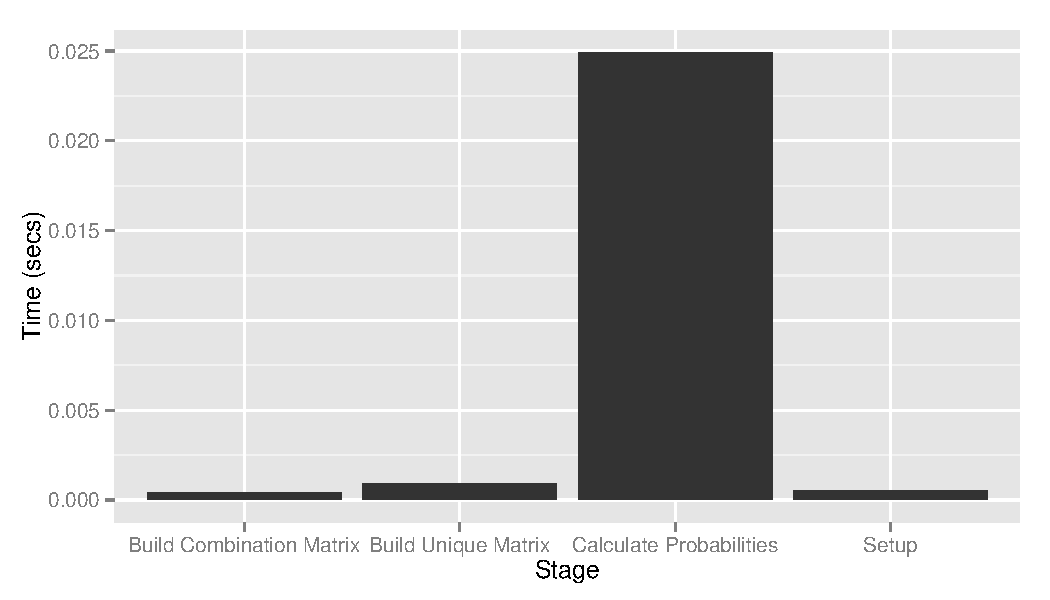
\includegraphics[width=6in]{getEventProbNr3.pdf}
	\caption{Timing of calling $getEventProb$ with $nr=3$ and three events specified}
	\label{getEventProbNr3}
\end{figure}

However, if the number of rolls increases but the length of events does not increase, the stage for building the unique matrix of combinations of roll sums becomes a major factor as well because it requires more time determine which permutations of the rolls are duplicates. Figure~\ref{getEventProbNr8} shows this timing.

\begin{figure}[h!]
	\centering
	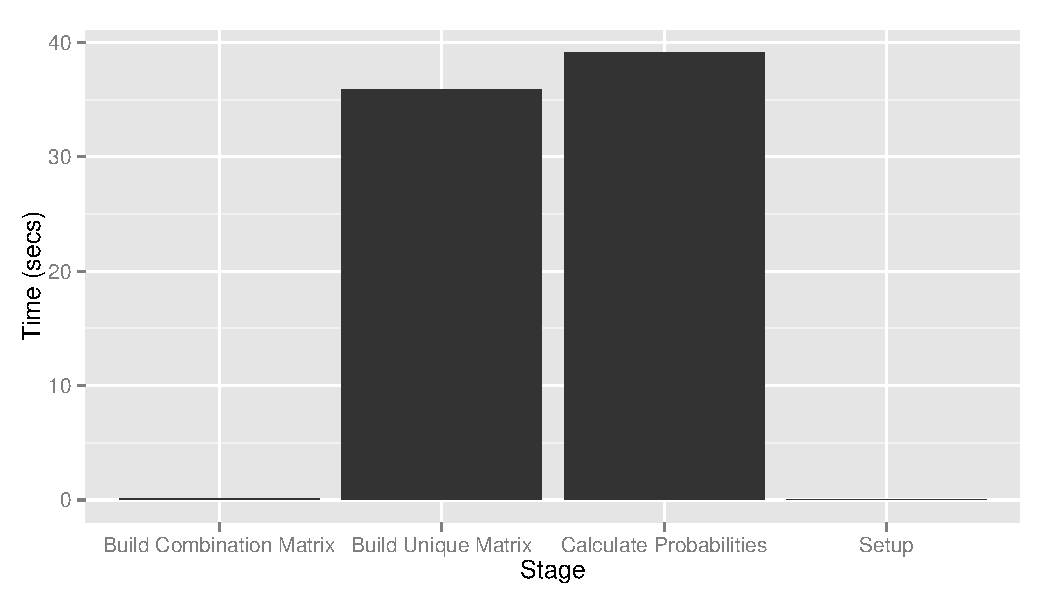
\includegraphics[width=6in]{getEventProbNr8.pdf}
	\caption{Timing of calling $getEventProb$ with $nr=8$ and three events specified}
	\label{getEventProbNr8}
\end{figure}

If the number of events specified is increased to match the roll count, then most of the time is spent again in calculating the probabilities as can be seen in Figure~\ref{getEventProbNr8Events8}. This is because the number of permutations is significantly lower.

\begin{figure}[h!]
	\centering
	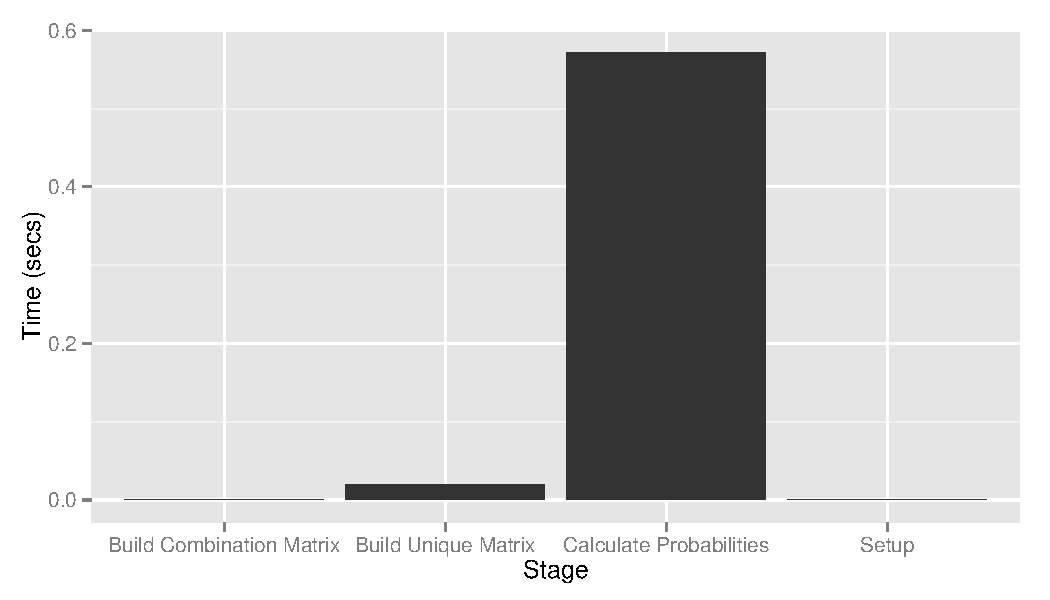
\includegraphics[width=6in]{getEventProbNr8Events8.pdf}
	\caption{Timing of calling $getEventProb$ with $nr=8$ and eight events specified}
	\label{getEventProbNr8Events8}
\end{figure}

Increasing the number of sides by die and the dice counts results in the same effect. By these graphs we can conclude that most of our efforts should be spent optimizing these two portions of the function $getEventProb$. These are namely the portion that computes the probabilities:

\begin{lstlisting}
sumOfProbs = sum(apply(combMatrix, 1,
	function(x) getEventProb(nrolls,
		ndicePerRoll,
		nsidesPerDie,
		as.list(x),
		orderMatters)))
\end{lstlisting}

and the portion that creates the unique matrix:

\begin{lstlisting}
if (nrolls > 1)
{
	combMatrix = unique(t(apply(combMatrix,1,sort)))
}
else
{
	combMatrix = unique(combMatrix)
}
\end{lstlisting}

\section{Code Optimization}

By examining the recursive call in calculating the $sumOfProbs$ in the previous section, we can see that there are many computations that are duplicated even though their results remain constant throughout the process of computing the total probability. Specifically, there are many repeated calls to $getSumProbs$ in $.getEventListProbs$. The function $getSumProbs$ only depends on $ndicePerRoll$ and $nsidesPerDie$ which does not change during the calculation, and it calculates the probability of each sum event. As a result, it can be cached and then reused. This significantly decreases the time required for the original code to execute when the number of dice increases as can be seen in Figure~\ref{codeOptimizations} for executing with the following arguments:

\begin{lstlisting}
getEventProb(nrolls=3, ndicePerRoll=rolls, nsidesPerDie=6,
	eventList=rep(list(rolls:(5*rolls)), 3), orderMatters=F)
\end{lstlisting}

\begin{figure}[h!]
	\centering
	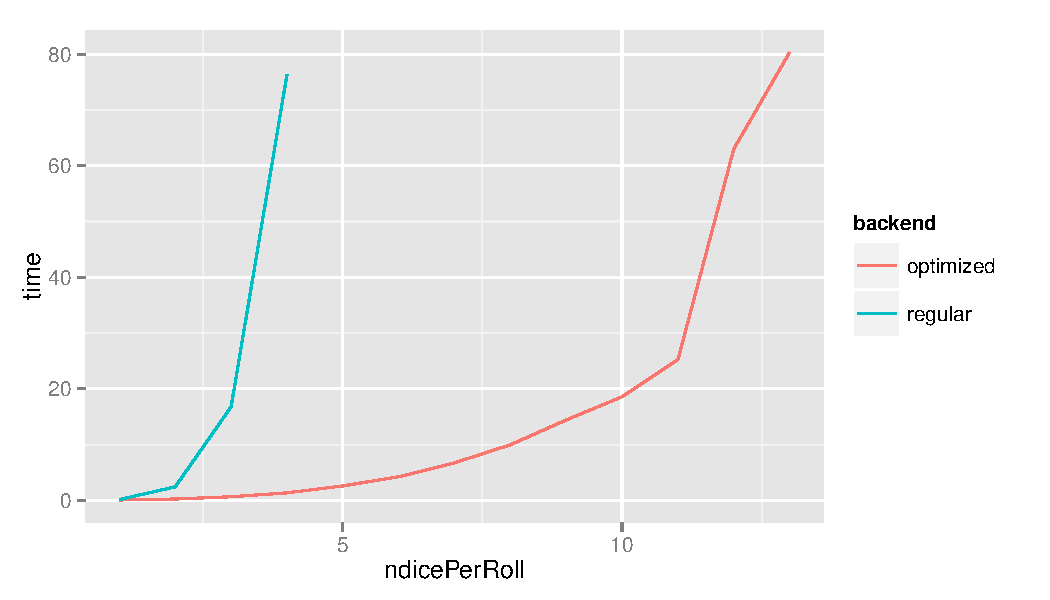
\includegraphics[width=6in]{codeOptimizations.pdf}
	\caption{Timing difference between original code and optimized version for number of dice}
	\label{codeOptimizations}
\end{figure}

Note that the event list is chosen to have a large range so that more computation is required. If the number of rolls is increased instead, then the optimizations do not have much effect on the execution time as can be seen in Figure~\ref{codeOptimizationsRolls}.

\begin{figure}[h!]
	\centering
	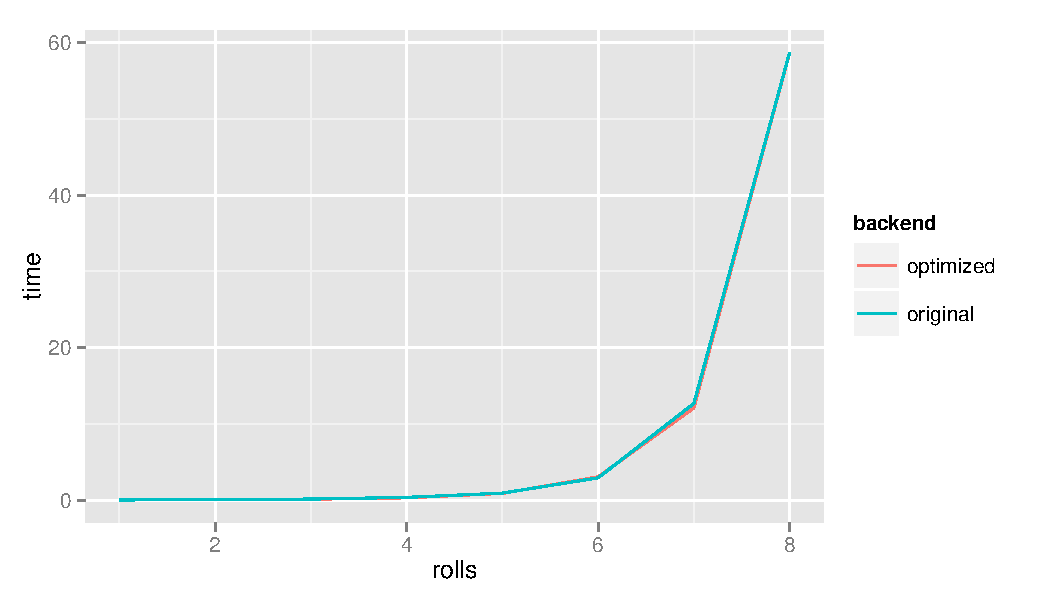
\includegraphics[width=6in]{codeOptimizationsRolls.pdf}
	\caption{Timing difference between original code and optimized version for number of rolls}
	\label{codeOptimizationsRolls}
\end{figure}

\section{Parallelizing Using $snow$}

As mentioned previously, most of the computation is done in the calculating of the probabilities, and these calculations are clearly independent from each other as the probability of each combination of rolls can be determined without information from the others. Therefore the code can be parallelized relatively easily by computing the probabilities of each combination in parallel using $parRapply$ from the $snow$ package \cite{snow}.

\begin{lstlisting}
probs = snowGetSumProbs(ndicePerRoll, nsidesPerDie)$probabilities
clusterExport(cls, c("snowGetEventProb",
	".snowGetEventListProbs", ".checkIntParam",
	".checkLogicalParam", "combinations"),
	envir=environment())
sumOfProbs = sum(parRapply(cls, combMatrix,
	function(x) {
		snowGetEventProb(nrolls,
			ndicePerRoll,
			nsidesPerDie,
			as.list(x),
			orderMatters,
			F,
			probs)
	}))
outcomeProb = sumOfProbs
\end{lstlisting}

This allows for the probability calculation stage to be spread over multiple cores. And yields slightly better performance as seen in Figure~\ref{snowComparison} for approximately $nDicePerRoll > 6$ and four cores. For around $nDicePerRoll <= 6$, the overhead incurred from synchronizing and transferring data to the cluster outweighs its gains from parallelization. However, even for the last case of thirteen dice, the difference in execution time is $(80.3\;sec -59.0\;sec)/80.3\;sec = 26.5\%$, which is significantly faster. This is because the work of calculating the probabilities of each row of $combMatrix$ can be divided across all the cores rather than only having one core do the calculations as in the original package code.

\begin{figure}[h!]
	\centering
	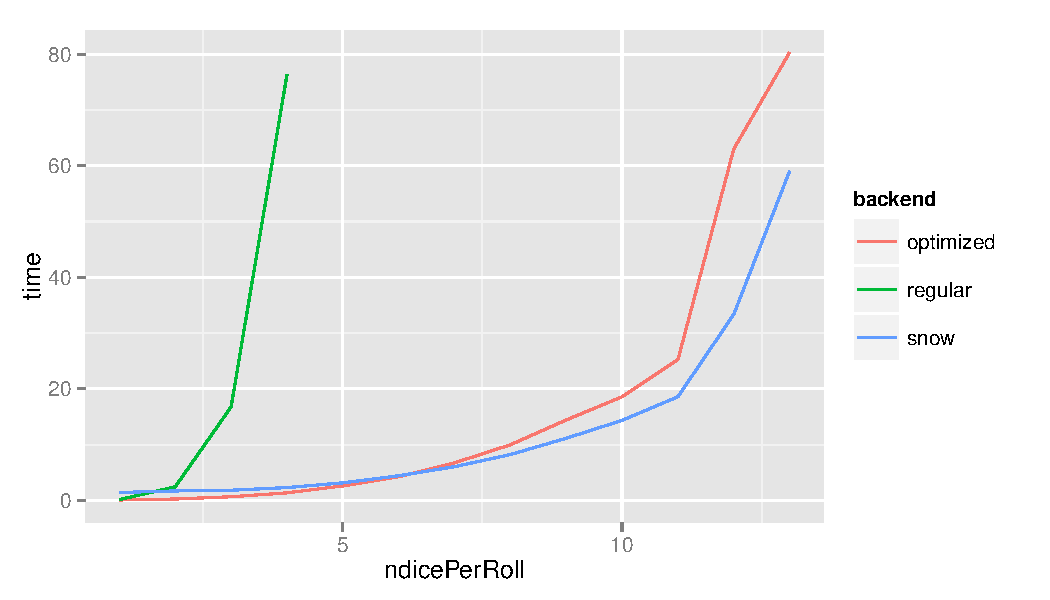
\includegraphics[width=6in]{snowComparison.pdf}
	\caption{Timing difference for code parallelized using $snow$}
	\label{snowComparison}
\end{figure}

Given how relatively trivial the use of $snow$ was, the performance improvements are very good. For the following parallelizations, it will require significantly more effort to port the current computations into C++ and parallelize the computation.

\section{Parallelizing Using OpenMP}

The OpenMP version of the algorithm works in a similar way by dividing the work by row to the different threads. On the main challenges here was reimplementing some of the package in C++ to be run more efficiently than in R. This re-writing improves the performance significantly as Figure~\ref{ompComparison} shows. A native implementation of the core part of the package helps speed things up. We had tried implementing all of the package in C++ but some of the algorithms used were difficult and error-prone to implement, so some of the code remained implemented in R. However, the portion still in R is not the bottleneck in the performance of the package.

The key points in the parallelization of the algorithm in OpenMP are the call to the C++ code:

\begin{lstlisting}
probs = ompGetSumProbs(ndicePerRoll, nsidesPerDie)$probabilities
sumOfProbs <- .Call("ompApplyGetEventProb", combMatrix, nrolls, probs[,2], ndicePerRoll, nsidesPerDie)
outcomeProb = sumOfProbs
\end{lstlisting}

and the C++ implementation of the calculation of each row probability:

\begin{lstlisting}
 #pragma omp parallel for schedule(static,1)	
 for(int i = 0; i < nrow; i++)
 {
	 sum[omp_get_thread_num()] += RowGetEventProb(ncol, c_nrolls, 
		 c_ndicePerRoll, c_nsidesPerDie, hv, passprob, i);
 }
\end{lstlisting}

\begin{figure}[h!]
	\centering
	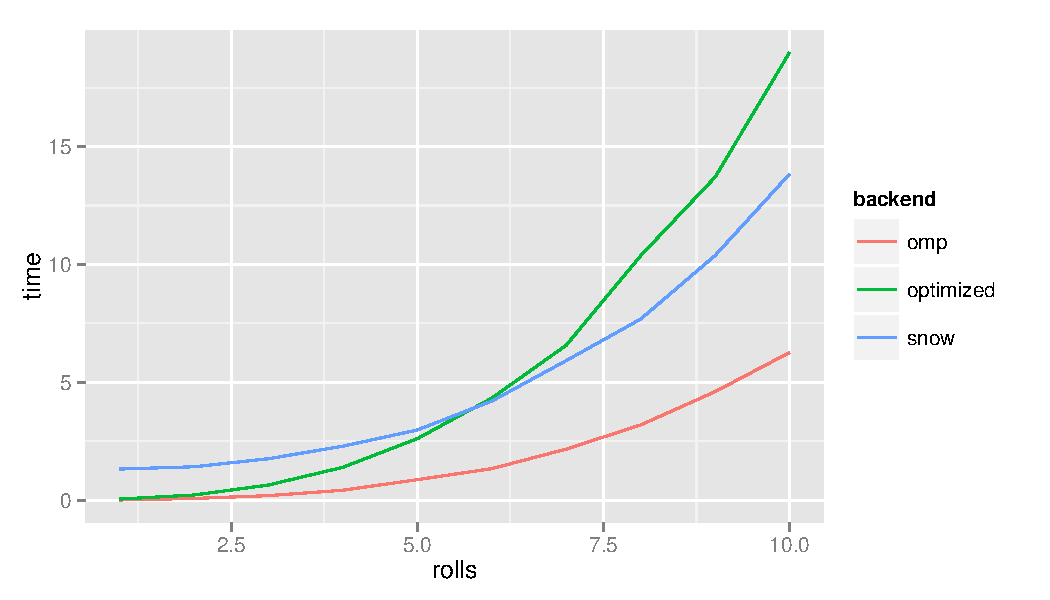
\includegraphics[width=6in]{ompComparison.pdf}
	\caption{Timing difference for code parallelized using $OpenMP$}
	\label{ompComparison}
\end{figure}

\section{Parallelizing Using Thrust}

The thrust \cite{thrust} version of the algorithm divides the work by row as in the snow case. It uses a C++ implementation of the probability calculation for each row as in the OpenMP version and performs significantly faster, especially since it's written in a lower level language compared to R. The following is where the transform and reduce occurs:

\begin{lstlisting}
thrust::device_vector<int> dm(size);
thrust::copy(hv.begin(), hv.end(), dm.begin());

thrust::host_vector<float> hprobs(probsM.size());
thrust::copy(probsM.begin(), probsM.end(), hprobs.begin());

thrust::device_vector<float> dprobs(size);
thrust::copy(hprobs.begin(), hprobs.end(), dprobs.begin());

thrust::device_vector<int> seq(nrow);
thrust::sequence(seq.begin(), seq.end());
thrust::device_vector<float> dv(nrow);
thrust::transform(seq.begin(), seq.end(),
	dv.begin(),
	RowGetEventProb(ncol, c_nrolls, 
		c_ndicePerRoll, c_nsidesPerDie, 
		dm.begin(), dprobs.begin()));
thrust::host_vector<float> host_prob(nrow);
thrust::copy(dv.begin(), dv.end(), dprobs.begin());

return wrap(thrust::reduce(dv.begin(), dv.end()));
\end{lstlisting}

And the functor has a similar implementation for calculating the probability for each individual row:

\begin{lstlisting}
struct RowGetEventProb
{
	int *combMat;
	float *probs;
	int ncol;
	int c_ndicePerRoll;
	int c_nsidesPerDie;
	int c_nrolls;
	
	RowGetEventProb(int ncol, int c_nrolls, int c_ndicePerRoll, int c_nsidesPerDie, thrust::device_vector<int>::iterator it_combMat, thrust::device_vector<float>::iterator it_probs)
	: ncol(ncol), c_nrolls(c_nrolls), c_ndicePerRoll(c_ndicePerRoll), 
	c_nsidesPerDie(c_nsidesPerDie)
	{
		combMat = thrust::raw_pointer_cast(&it_combMat[0]);
		probs = thrust::raw_pointer_cast(&it_probs[0]);
	}
	
	__device__ float operator()(const int& matrix_i)
	{
		// See Appendix for code listing
	}
};

\end{lstlisting}

The performance comparison can be seen in Figure~\ref{thrustComparison} with parallelism of four cores:

\begin{figure}[h!]
	\centering
	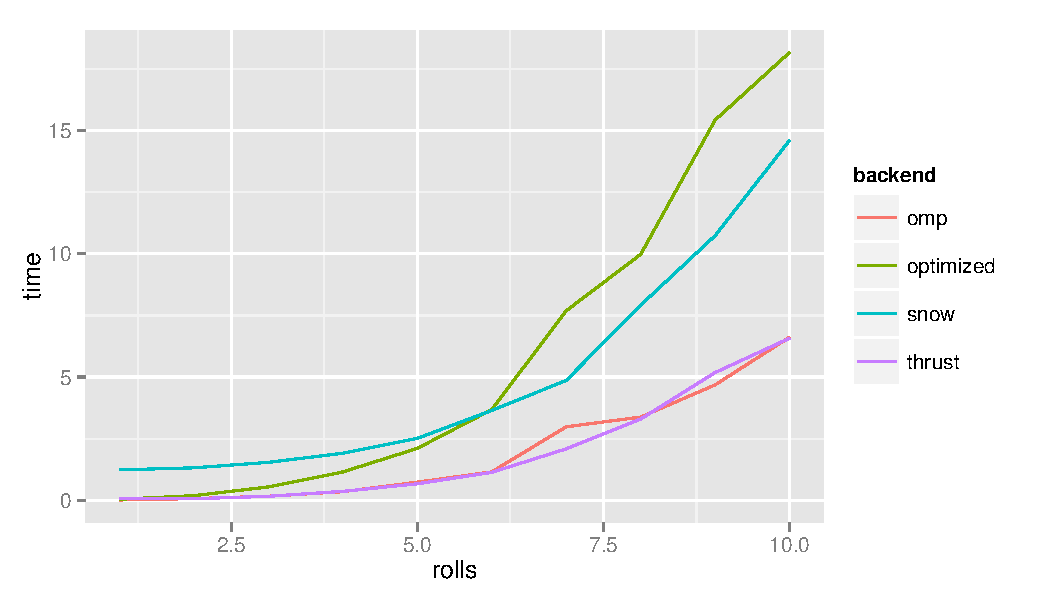
\includegraphics[width=6in]{thrustComparison.pdf}
	\caption{Timing difference for code parallelized using $thrust$}
	\label{thrustComparison}
\end{figure}

Clearly the $thrust$ implementation did not have much of an effect over the direct OpenMP implementation. This shows that the abstraction of $thrust$ does have some overhead, but it was not significant in this case. In other words it provided pretty good parallelism despite being at a higher level.

\section{Results}

After applying $snow$, OpenMP and $thrust$ to the $dice$ package we saw strong improvements over the non-parallel dice package. Snow provided the
least increase in performance with a average close to the optimized version of $dice.R$. Due to snow's communication between nodes in clusters 
some performance was lost thus taking up almost as much time as the actual function. Many of the calculations preformed by $getEventList$ and $getSumProbs$
are short and non-intensive thus providing snow with less time to achieve any meaning full speed up before having to communicate with nodes again and handling 
data that must be returned. Thrust with an OpenMP backend along with OpenMP provided about a 75\% decrease in computation time. Thrust was able to
remove the bottle neck within $dice.R$ and $dice.cpp$ by calculation probabilities based on different rows of the $combMatrix$. This was achieved by 
creating a functor $RowGetEventProb$ which used a device kernel to perform probability calculations on the GPU at a very fast rate since the machines 
being used to run the code have GPUs with 192 CUDA cores. The OpenMP version also took advantage of the fact that the recursion on the combMatrix was the
main bottleneck for the original package. Thus by chunking the rows and passing them to multiple cores we were able to achieve a strong performance increase
and allowing each CPU to work on a contiguous block of $combMatrix$ thus each CPU is working on non-shared data and avoiding false sharing which happens 
when data shared by multiple CPUs is modified frequently. Also, OpenMP takes a more relaxed consistency approach, forcing updates at all synchronization points
\cite{matloff_parallel}, which can provide for an increase in performance compared to the other models. After applying snow, OpenMP and thrust to the dice 
package we saw strong improvments over the non-parrallel dice package.

\appendix

\section{Code Listings}

\subsection{$snow$}

This contains the $snow$ implementation of the dice package. The key point is the location that uses $parRapply$ on the cluster to parallelize the computation. Also note the caching the probabilities sums and passing that data rather than recomputing it for each row.

\begin{lstlisting}

library(gtools)
library(parallel)
library(dice)
library(ggplot2)

# @@@@@@@@@@@@@@@@@@@@@@@@@@@@@@@@@@@@@@@@@@@@@@@@@@@@@@@@@@@@@@@@@@@@@@@@@@@@@@@@@@@@


# These helper functions check parameter integrity

.checkIntParam = function(param, paramName, positive)
{
  if ((!missing(positive) && param < (if (positive) 1 else 0)) ||
        (param != floor(param)) ||
        (length(param) > 1))
  {
    if (missing(positive))  
    {
      paste("\n*", paramName, "must contain a single integer instead of", param)
    }
    else if (positive)
    {
      paste("\n*", paramName, "must contain a single positive integer instead of", param)
    }
    else 
    {
      paste("\n*", paramName, "must contain a single non-negative integer instead of", param)
    }
  }
}


.checkLogicalParam = function(param, paramName)
{
  if (length(param) > 1 ||
        !is.logical(param))
  {
    paste("\n* ", paramName, " must contain a single logical value (i.e., TRUE or FALSE)", sep="")
  }
}


# This helper function returns the probabilities of each element of eventList

.snowGetEventListProbs = function(ndicePerRoll, nsidesPerDie, eventList, probs)
{
  
  # On the assumption that eventList has length nrolls (which is safe since this is a 
  # private helper function), we calculate the probability of getting an acceptable 
  # outcome (a "success") on each of the rolls by iterating through the vector of 
  # successes for that roll and adding the corresponding probability to our tally
  
  eventListProbs = c()
  for (i in 1:length(eventList)) 
  {
    successesForThisRoll = sort(eventList[[i]])
    successProbForThisRoll = 0
    for (j in 1:length(successesForThisRoll))
    {
      successProbForThisRoll = successProbForThisRoll + probs[(successesForThisRoll[j] - (ndicePerRoll - 1)),2]
    }
    eventListProbs[i] = successProbForThisRoll
  }
  eventListProbs 
}


checkpoint <- function(marker, message) {
  newMarker <- Sys.time()
  print(message)
  print(newMarker - marker)
  return(newMarker)
}

# @@@@@@@@@@@@@@@@@@@@@@@@@@@@@@@@@@@@@@@@@@@@@@@@@@@@@@@@@@@@@@@@@@@@@@@@@@@@@@@@@@@@


# NOTE: the parameters nrolls, ndicePerRoll, nsidesPerDie, and nkept in the function
# signatures below depart slightly from our usual coding conventions (i.e., are not 
# numRolls, numDicePerRoll, numSidesPerDie, and numDiceKept) so that they are easily 
# abbreviated as "nr", "nd", "ns", and "nk", respectively, in function calls

snowGetEventProb = function(nrolls,
                            ndicePerRoll,
                            nsidesPerDie,
                            eventList,
                            orderMatters=FALSE,
                            top=F,
                            probs=NULL,
                            parallel=4)
{
  marker <- Sys.time()
  
  errorVector = character()
  errorVector = append(errorVector, .checkIntParam(nrolls, "nrolls", positive=TRUE))
  errorVector = append(errorVector, .checkIntParam(ndicePerRoll, "ndicePerRoll", positive=TRUE))
  errorVector = append(errorVector, .checkIntParam(nsidesPerDie, "nsidesPerDie", positive=TRUE))
  
  if (length(eventList) > nrolls)
  {
    errorVector = append(errorVector, "\n* The length of eventList must not be greater than nrolls")
  }
  if (orderMatters & length(eventList) != nrolls)
  {
    errorVector = append(errorVector, "\n* If orderMatters is passed as TRUE, the length of eventList must equal\n  nrolls (i.e., there must be an element of eventList for each roll)")
  }
  if (!all(sapply(eventList, is.numeric)))
  {
    errorVector = append(errorVector, "\n* All elements of eventList must be numeric vectors")
  }
  if (!all(as.logical(sapply(sapply(eventList, function(x) x == floor(x)), min))))
  {
    errorVector = append(errorVector, "\n* All numbers in each element of eventList must be positive integers")
  }
  if (min(sapply(eventList, min)) < ndicePerRoll ||
        max(sapply(eventList, max)) > (ndicePerRoll * nsidesPerDie))
  {
    errorVector = append(errorVector, "\n* All numbers in each element of eventList must be between ndicePerRoll\n  and (ndicePerRoll * nsidesPerDie)")
  }
  errorVector = append(errorVector, .checkLogicalParam(orderMatters, "orderMatters"))
  
  if (length(errorVector) > 0)
  {
    stop(errorVector)
  }
  
  eventList = lapply(eventList, unique)
  
  # If eventList doesn't have an element for each roll, we add elements until it does;
  # after this point, each element of eventList will constrain one roll (but some of 
  # those constraints may be simply {min:max} for that roll--i.e., trivial constraints)
  
  if (length(eventList) < nrolls)
  {
    eventList = lapply(c(eventList, rep(0, nrolls - length(eventList))), function(x){x = (if (max(x) == 0) ndicePerRoll:(ndicePerRoll*nsidesPerDie) else x)})    
  }
  
  if (orderMatters)
  {
    if(is.null(probs)){
      probs = snowGetSumProbs(ndicePerRoll, nsidesPerDie)$probabilities
    }
    outcomeProb = prod(.snowGetEventListProbs(ndicePerRoll, nsidesPerDie, eventList, probs))
  }
  else # i.e., if (!orderMatters)
  {
    if(top)
      marker <- checkpoint(marker, "Set up")
    # We only calculate probabilities if each element of eventList is a length-1 vector
    # (i.e., a single number), e.g., {2, 3, 2}; if any element is longer than that, e.g.,
    # {2, {3, 4}, 2}, we call ourselves recursively on each list we can construct of only
    # length-1 vectors (e.g., in the example above we'd call ourselves on {2, 3, 2} and 
    # {2, 4, 2}); then we sum the resulting probabilities (which, since orderMatters is 
    # FALSE, account for all permutations of each of {2, 3, 2} and {2, 4, 2}) to arrive 
    # at our probability for the original list of {2, {3, 4}, 2}
    
    listElemLengths = sapply(eventList, length)
    maxListElemLength = max(listElemLengths)
    if(top)
      marker <- checkpoint(marker, "MaxList")
    if (maxListElemLength > 1)
    {
      # Here we populate combMatrix with the elements of eventList to produce a 
      # matrix each row of which is a selection of one element from each element of
      # eventList; e.g., given the eventList {{1, 2}, {1, 2, 4}, 2}, we'd produce
      # a 6 x 3 matrix with rows {1, 1, 2}, {1, 2, 2}, {1, 4, 2}, {2, 1, 2}, {2, 2, 2},
      # and {2, 4, 2}
      
      combMatrix = matrix(nrow = prod(listElemLengths), ncol = nrolls)
      if (nrolls > 1)
      {
        for (i in 1:(nrolls-1))
        {
          combMatrix[,i] = rep(eventList[[i]], each = prod(listElemLengths[(i+1):nrolls]))
        }
      }
      combMatrix[,nrolls] = rep(eventList[[nrolls]])
      
      if(top)
        marker <- checkpoint(marker, "Comb")
      
      # Next we eliminate all rows that are permutations of other rows (otherwise we
      # would over-count in the calculations that follow)
      
      if (nrolls > 1)
      {
        combMatrix = unique(t(apply(combMatrix,1,sort)))
      }
      else
      {
        combMatrix = unique(combMatrix)
      }
      
      if(top)
        marker <- checkpoint(marker, "Unique")
      
      # Now we make a recursive call for each row of combMatrix and sum the resulting
      # probabilities to arrive at our probability for the original eventList
      # Create cluster
      cls <- makePSOCKcluster(rep("localhost", parallel))
      probs = snowGetSumProbs(ndicePerRoll, nsidesPerDie)$probabilities
      # Export functions
      clusterExport(cls, c("snowGetEventProb", ".snowGetEventListProbs", ".checkIntParam", ".checkLogicalParam", "combinations"),
                    envir=environment())
      # Apply in parallel
      result <- parRapply(cls, combMatrix,
                function(x) {
                  snowGetEventProb(nrolls,
                                   ndicePerRoll,
                                   nsidesPerDie,
                                   as.list(x),
                                   orderMatters,
                                   F,
                                   probs)
                })
      # Reduce into sum
      sumOfProbs = sum(result)
      outcomeProb = sumOfProbs
      stopCluster(cls)
      
      if(top)
        marker <- checkpoint(marker, "Sum")
    }
    else
    {
      # If each element of eventList is a length-1 vector, we can convert eventList
      # itself to a vector; then we calculate the probability of getting the specific
      # set of outcomes specified by eventList in any order (reflecting the fact that 
      # orderMatters was passed in as FALSE)
      
      eventListAsVector = sapply(eventList, max)
      eventListProb = prod(.snowGetEventListProbs(ndicePerRoll, nsidesPerDie, eventListAsVector, probs))
      outcomeProb = eventListProb * factorial(nrolls) / prod(factorial(table(eventListAsVector)))
    }
  }
  
  outcomeProb
}

# @@@@@@@@@@@@@@@@@@@@@@@@@@@@@@@@@@@@@@@@@@@@@@@@@@@@@@@@@@@@@@@@@@@@@@@@@@@@@@@@@@@@


snowGetSumProbs = function(ndicePerRoll,
                       nsidesPerDie,
                       nkept = ndicePerRoll,
                       dropLowest = TRUE,
                       sumModifier = 0,
                       perDieModifier = 0,
                       perDieMinOfOne = TRUE)
{
  
  # We begin with preliminary error-checking
  
  errorVector = vector(mode = "character", length = 0)
  errorVector = append(errorVector, .checkIntParam(ndicePerRoll, "ndicePerRoll", positive=TRUE))
  errorVector = append(errorVector, .checkIntParam(nsidesPerDie, "nsidesPerDie", positive=TRUE))
  errorVector = append(errorVector, .checkIntParam(nkept, "nkept", positive=TRUE))
  if (nkept > ndicePerRoll)
  {
    errorVector = append(errorVector, "\n* nkept must not be greater than ndicePerRoll")
  }
  errorVector = append(errorVector, .checkIntParam(sumModifier, "sumModifier"))
  errorVector = append(errorVector, .checkIntParam(perDieModifier, "perDieModifier"))
  errorVector = append(errorVector, .checkLogicalParam(perDieMinOfOne, "perDieMinOfOne"))
  
  if (length(errorVector) > 0)
  {
    stop(errorVector)
  }
  
  numOutcomes = nsidesPerDie^ndicePerRoll
  numDiceToDrop = ndicePerRoll - nkept
  currNumArrangements = 0
  
  sumModifier = sumModifier + (perDieModifier * nkept)
  
  currentSum = 0
  
  vectorOfSums = as.integer((nkept + sumModifier) :
                              ((nsidesPerDie * nkept) + sumModifier))
  
  numPossibleSums = length(vectorOfSums)
  
  # sumTallyMatrix is used to track the number of times we see every possible outcome sum,
  # which we will use to produce the probabilities of every sum (e.g., for the 3d6 case we 
  # see 10 as a sum 27 times, so the probability of a sum of 10 is 27/216 = .125, while for
  # the 5d6 drop 2 case we see 13 as a sum 1055 times, so the probability of a sum of 13
  # is 1055/7776 = .1356739).
  
  sumTallyMatrix = matrix(data = c(vectorOfSums,
                                   as.integer(rep.int(0, numPossibleSums)),
                                   as.integer(rep.int(0, numPossibleSums))),
                          nrow = numPossibleSums,
                          ncol = 3,
                          dimnames = list(NULL,
                                          c("Sum",
                                            "Probability",
                                            "Ways to Roll")))
  
  # boundaryVal is the most extreme die-roll value that will be kept (i.e., the die-roll "boundary"
  # value: e.g., for 5d6 drop lowest two, if our sorted die rolls are {3 4 4 5 6}, boundaryVal is 4).
  # We'll call all dice with this value the "b" dice (because they're on the [b]oundary).
  
  for (boundaryVal in 1 : nsidesPerDie)
  {
    
    # numOs is the number of dice whose values are outside of boundaryVal (e.g., for 5d6 drop lowest 
    # two, if we roll {3 4 4 5 6}, boundaryVal is 4, so numOs is 1).  We'll call these dice the "o"
    # dice (because they're [o]utside our boundary).  
    # NOTE: We have an embedded if clause in our for-loop declaration because if we're dropping lowest 
    # and boundaryVal is 1 or we're dropping highest and boundaryVal is nsidesPerDie, there cannot be 
    # any dice whose values are outside of boundaryVal, and hence numOs can only be 0.  The following 
    # loop syntax might look suspicious, but we *do* want to iterate once in these two cases, as well
    # as in the case where numDiceToDrop is 0 (and in all three such cases, numOs will be 0).
    
    for (numOs in 0 : (if ((dropLowest && boundaryVal == 1) ||
                             (!dropLowest && boundaryVal == nsidesPerDie)) 0 else numDiceToDrop))
    {
      
      # numBsKept is the number of b's that will be kept (e.g., for 5d6 drop lowest two, if we roll
      # {3 4 4 5 6}, numBsKept is 1, because one of the two 4's will be kept).
      # Now, since we're discarding numDiceToDrop dice (including the numOs o's), we'll discard 
      # (numDiceToDrop - numOs) of the b's and keep numBsKept of them, and thus the total number of
      # b's is (numBsKept + numDiceToDrop - numOs).  NOTE: Hence, the number of dice whose values
      # exceed boundaryVal is (nkept - numBsKept).  We will call these higher dice the "i" dice (since
      # they're "inside" our boundary).
      
      for (numBsKept in 1 : nkept)
      {
        
        # By this part of the function, we've specified a class of outcomes identified by their 
        # (boundaryVal, numOs, numBsKept) values--i.e., every outcome in this class has the
        # following properties:
        # 1). the die-roll boundary value boundaryVal; 
        # 2). numOs "o" dice, whose values are outside boundaryVal and will be dropped; and
        # 3). numBsKept "b" dice that will be kept.  Furthermore, each such outcome has
        # 4). (numBsKept + numDiceToDrop - numOs) "b" dice in total, and 
        # 5). (nkept - numBsKept) "i" dice, whose values are inside boundaryVal.
        
        numBs = (numBsKept + numDiceToDrop - numOs)
        numIs = (nkept - numBsKept)
        
        paste("\n\nIn this class, boundaryVal is ", boundaryVal, ", numOs is ", numOs,", numBsKept is", numBsKept, ", numBs is ", numBs, ", and numIs is ", numIs, "\n", sep="")
        
        # Now, we're interested in sums for the various outcomes in this class, and these sums
        # don't depend upon the order in which the various values appear in our sequence of
        # rolls; i.e., multiple outcomes in this class will have the same values but have the o's,
        # the b's, and the i's appear at different places in the sequence of rolls.  To account
        # for this, we need to multiply each distinct outcome by the number of other outcomes
        # that are identical to it except for the order in which the o's, b's, and i's occur
        # (NOTE: the orders *within* these groups are accounted for below: order within the o's 
        # is accounted for immediately below, and we account for the order within the i's in the
        # section of the code in which we enumerate the i's).  For now, we will define a term by
        # which to multiply each sum we find; this term is a result of the multinomial theorem's 
        # combinatoric interpretation as the number of ways to put n distinct objects (in this 
        # case, our die rolls) into 3 bins of size numOs, (numBsKept + numDiceToDrop - numOs), 
        # and (nkept - numBsKept), corresponding to the number of o's, b's, and i's in the class:
        
        numArrangementsOfDice = (factorial(ndicePerRoll) / 
                                   (factorial(numOs) * factorial(numBs) * factorial(numIs)))
        
        # [NOTE: The formula above could overflow if ndicePerRoll gets large, in which case we may
        #  consider using lfactorial()--but I think the function would keel over before then anyway]
        
        # Because we support dropping lowest or highest values, we define convenient variables
        # to allow us to operate over appropriate ranges for the rest of this function
        
        innerBoundary = if (dropLowest) nsidesPerDie else 1
        outerBoundary = if (dropLowest) 1 else nsidesPerDie
        rangeOfOVals = abs(boundaryVal - outerBoundary)
        rangeOfIVals = abs(boundaryVal - innerBoundary)
        possibleIValsVec = if (dropLowest) ((boundaryVal+1) : nsidesPerDie) else (1 : (boundaryVal-1))
        
        # Next: The value of boundaryVal is fixed for this loop, but there are many "o" dice values
        # that outcomes in this class might have; because we don't care about these values, we need
        # to increase our multiplicity term to account for the outcomes that will be identical 
        # to this iteration's distinct outcome but for the values (and order) of the o's:
        
        numArrangementsOfDice = numArrangementsOfDice * rangeOfOVals^numOs
        
        # Now that we've accounted for sorting the values into three bins and for all the possible
        # "o" values that are immaterial to our calculations, we can treat our outcome class as
        # sorted into groups and can focus our attention on the numBsKept b's we keep and the 
        # i's.  The numBsKept b's will contribute a known amount to our sum for all outcomes in 
        # this class (viz., numBsKept * boundaryVal); but the i's will contribute various amounts, 
        # depending on their values.  So now we turn to determining the possible distinct outcomes 
        # for this class by enumerating the possible values for the i's.  We will work as follows:
        # rangeOfIVals is the distance between the smallest and largest possible "i" values for this
        # class of outcomes, and we use it to determine the number of distinct outcomes for this
        # class, which is given by rangeOfIVals^numIs.  We create an outcomeMatrix with as many
        # rows as there are distinct outcomes for this class and nkept columns; each element
        # in a row corresponds to a die-roll value, and the sum of the row elements is the
        # sum for that distinct outcome.  We populate outcomeMatrix with a row for every possible 
        # value for the i's in this class (and hence all distinct outcomes in the class).  We then
        # calculate the number of permutations of each distinct outcome (e.g., in the 3d6 case,
        # the outcome {1, 1, 2} has three permutations) and use this information to calculate the 
        # probability of every possible outcome in this class.
        
        if (numBsKept == nkept)
        {
          currentSum = (numBsKept * boundaryVal) + sumModifier
          # We adjust row index by (nkept - 1) so that, e.g., a 3d6 tally starts in row 1, not 3
          sumTallyMatrix[currentSum - sumModifier - (nkept - 1), 2] = sumTallyMatrix[currentSum - sumModifier - (nkept - 1), 2] + numArrangementsOfDice
        }
        else
        {
          outcomeMatrix = matrix(nrow = choose((rangeOfIVals + numIs - 1), numIs), ncol = nkept)
          
          if (dim(outcomeMatrix)[1] > 0)
          {
            
            outcomeMatrix[,1 : numBsKept] = boundaryVal
            
            hCombs = combinations(n = rangeOfIVals,
                                  r = numIs,
                                  v = possibleIValsVec,
                                  repeats.allowed = TRUE)
            hPermCounts = apply(hCombs, 1, function(x) factorial(numIs)/prod(factorial(table(x))))
            
            outcomeMatrix[,(numBsKept+1) : nkept] = hCombs
            
            for (rowNum in 1 : nrow(outcomeMatrix))
            {
              currentSum = sum(outcomeMatrix[rowNum,]) + sumModifier
              currNumArrangements = numArrangementsOfDice * hPermCounts[rowNum]
              sumTallyMatrix[currentSum - sumModifier - (nkept - 1), 2] = sumTallyMatrix[currentSum - sumModifier - (nkept - 1), 2] + currNumArrangements
            }
          }
        }
      }
    }
  }
  
  if (perDieMinOfOne)
  {
    if (sumTallyMatrix[numPossibleSums,1] <= nkept)
    {
      sumTallyMatrix = matrix(data = c(nkept, numOutcomes, numOutcomes),
                              nrow = 1,
                              ncol = 3,
                              dimnames = list(NULL,
                                              c("  Sum  ","  Probability  ", "  Ways to Roll  ")))
    }
    else
    {
      extraWaysToRollMin = sum(sumTallyMatrix[sumTallyMatrix[,1] < nkept,2])
      sumTallyMatrix = sumTallyMatrix[sumTallyMatrix[,1] >= nkept,]
      sumTallyMatrix[1,2] = sumTallyMatrix[1,2] + extraWaysToRollMin
    }
  }
  
  sumTallyMatrix[,3] = sumTallyMatrix[,2]
  sumTallyMatrix[,2] = sumTallyMatrix[,2] / numOutcomes
  
  overallAverageSum = sum(sumTallyMatrix[,1] * sumTallyMatrix[,3] / numOutcomes)
  
  list(probabilities = sumTallyMatrix, average = overallAverageSum)
}
\end{lstlisting}

\subsection{Optimized}

This contains the optimized implementation of the dice package. Note the caching the probabilities sums and passing that data rather than recomputing it for each row which improves performance

\begin{lstlisting}
library(gtools)

# @@@@@@@@@@@@@@@@@@@@@@@@@@@@@@@@@@@@@@@@@@@@@@@@@@@@@@@@@@@@@@@@@@@@@@@@@@@@@@@@@@@@


# These helper functions check parameter integrity

.checkIntParam = function(param, paramName, positive)
{
  if ((!missing(positive) && param < (if (positive) 1 else 0)) ||
        (param != floor(param)) ||
        (length(param) > 1))
  {
    if (missing(positive))  
    {
      paste("\n*", paramName, "must contain a single integer instead of", param)
    }
    else if (positive)
    {
      paste("\n*", paramName, "must contain a single positive integer instead of", param)
    }
    else 
    {
      paste("\n*", paramName, "must contain a single non-negative integer instead of", param)
    }
  }
}


.checkLogicalParam = function(param, paramName)
{
  if (length(param) > 1 ||
        !is.logical(param))
  {
    paste("\n* ", paramName, " must contain a single logical value (i.e., TRUE or FALSE)", sep="")
  }
}

# This helper function returns the probabilities of each element of eventList

.optGetEventListProbs = function(ndicePerRoll, nsidesPerDie, eventList, probs)
{
  
  # On the assumption that eventList has length nrolls (which is safe since this is a 
  # private helper function), we calculate the probability of getting an acceptable 
  # outcome (a "success") on each of the rolls by iterating through the vector of 
  # successes for that roll and adding the corresponding probability to our tally
  
  #cat("E", eventList)
  #print(probs)
  eventListProbs = c()
  for (i in 1:length(eventList)) 
  {
    successesForThisRoll = sort(eventList[[i]])
    successProbForThisRoll = 0
    for (j in 1:length(successesForThisRoll))
    {
#        cat("D", (successesForThisRoll[j] - (ndicePerRoll - 1)))
       #cat("P", probs[(successesForThisRoll[j] - (ndicePerRoll - 1)),2])
#      print(ndicePerRoll)
        #cat("P", ndicePerRoll)
      #print("P")
      successProbForThisRoll = successProbForThisRoll + probs[(successesForThisRoll[j] - (ndicePerRoll - 1)),2]
    }
    eventListProbs[i] = successProbForThisRoll
  }
  #cat("H", eventListProbs[i], "\n")
  eventListProbs 
}

optGetEventProb = function(nrolls,
                           ndicePerRoll,
                           nsidesPerDie,
                           eventList,
                           orderMatters=FALSE,
                           top=F,
                           probs=NULL)
{
  marker <- Sys.time()
  
  errorVector = character()
  errorVector = append(errorVector, .checkIntParam(nrolls, "nrolls", positive=TRUE))
  errorVector = append(errorVector, .checkIntParam(ndicePerRoll, "ndicePerRoll", positive=TRUE))
  errorVector = append(errorVector, .checkIntParam(nsidesPerDie, "nsidesPerDie", positive=TRUE))
  
  if (length(eventList) > nrolls)
  {
    errorVector = append(errorVector, "\n* The length of eventList must not be greater than nrolls")
  }
  if (orderMatters & length(eventList) != nrolls)
  {
    errorVector = append(errorVector, "\n* If orderMatters is passed as TRUE, the length of eventList must equal\n  nrolls (i.e., there must be an element of eventList for each roll)")
  }
  if (!all(sapply(eventList, is.numeric)))
  {
    errorVector = append(errorVector, "\n* All elements of eventList must be numeric vectors")
  }
  if (!all(as.logical(sapply(sapply(eventList, function(x) x == floor(x)), min))))
  {
    errorVector = append(errorVector, "\n* All numbers in each element of eventList must be positive integers")
  }
  if (min(sapply(eventList, min)) < ndicePerRoll ||
        max(sapply(eventList, max)) > (ndicePerRoll * nsidesPerDie))
  {
    errorVector = append(errorVector, "\n* All numbers in each element of eventList must be between ndicePerRoll\n  and (ndicePerRoll * nsidesPerDie)")
  }
  errorVector = append(errorVector, .checkLogicalParam(orderMatters, "orderMatters"))
  
  if (length(errorVector) > 0)
  {
    stop(errorVector)
  }
  
  if(is.null(probs)){
    probs = optGetSumProbs(ndicePerRoll, nsidesPerDie)$probabilities
    #print(probs)
  }
  
  eventList = lapply(eventList, unique)
  
  # If eventList doesn't have an element for each roll, we add elements until it does;
  # after this point, each element of eventList will constrain one roll (but some of 
  # those constraints may be simply {min:max} for that roll--i.e., trivial constraints)
  
  if (length(eventList) < nrolls)
  {
    eventList = lapply(c(eventList, rep(0, nrolls - length(eventList))), function(x){x = (if (max(x) == 0) ndicePerRoll:(ndicePerRoll*nsidesPerDie) else x)})    
  }
  
  if (orderMatters)
  {
    outcomeProb = prod(.optGetEventListProbs(ndicePerRoll, nsidesPerDie, eventList, probs))
  }
  else # i.e., if (!orderMatters)
  {
    if(top)
      marker <- checkpoint(marker, "Set up")
    # We only calculate probabilities if each element of eventList is a length-1 vector
    # (i.e., a single number), e.g., {2, 3, 2}; if any element is longer than that, e.g.,
    # {2, {3, 4}, 2}, we call ourselves recursively on each list we can construct of only
    # length-1 vectors (e.g., in the example above we'd call ourselves on {2, 3, 2} and 
    # {2, 4, 2}); then we sum the resulting probabilities (which, since orderMatters is 
    # FALSE, account for all permutations of each of {2, 3, 2} and {2, 4, 2}) to arrive 
    # at our probability for the original list of {2, {3, 4}, 2}
    
    listElemLengths = sapply(eventList, length)
    maxListElemLength = max(listElemLengths)
    if(top)
      marker <- checkpoint(marker, "MaxList")
    if (maxListElemLength > 1)
    {
      # Here we populate combMatrix with the elements of eventList to produce a 
      # matrix each row of which is a selection of one element from each element of
      # eventList; e.g., given the eventList {{1, 2}, {1, 2, 4}, 2}, we'd produce
      # a 6 x 3 matrix with rows {1, 1, 2}, {1, 2, 2}, {1, 4, 2}, {2, 1, 2}, {2, 2, 2},
      # and {2, 4, 2}
      
      combMatrix = matrix(nrow = prod(listElemLengths), ncol = nrolls)
      if (nrolls > 1)
      {
        for (i in 1:(nrolls-1))
        {
          combMatrix[,i] = rep(eventList[[i]], each = prod(listElemLengths[(i+1):nrolls]))
        }
      }
      combMatrix[,nrolls] = rep(eventList[[nrolls]])
      
      if(top)
        marker <- checkpoint(marker, "Comb")
      
      # Next we eliminate all rows that are permutations of other rows (otherwise we
      # would over-count in the calculations that follow)
      
      if (nrolls > 1)
      {
        combMatrix = unique(t(apply(combMatrix,1,sort)))
      }
      else
      {
        combMatrix = unique(combMatrix)
      }
      
      if(top)
        marker <- checkpoint(marker, "Unique")
      
      # Now we make a recursive call for each row of combMatrix and sum the resulting
      # probabilities to arrive at our probability for the original eventList
      sumOfProbs = sum(apply(combMatrix, 1,
                             function(x) optGetEventProb(nrolls,
                                                          ndicePerRoll,
                                                          nsidesPerDie,
                                                          as.list(x),
                                                          orderMatters,
                                                          F,
                                                          probs)))
      outcomeProb = sumOfProbs
      
      if(top)
        marker <- checkpoint(marker, "Sum")
      
      #print("Recursed")
    }
    else
    {
      # If each element of eventList is a length-1 vector, we can convert eventList
      # itself to a vector; then we calculate the probability of getting the specific
      # set of outcomes specified by eventList in any order (reflecting the fact that 
      # orderMatters was passed in as FALSE)
      
      eventListAsVector = sapply(eventList, max)
      eventListProb = prod(.optGetEventListProbs(ndicePerRoll, nsidesPerDie, eventListAsVector, probs))
      outcomeProb = eventListProb * factorial(nrolls) / prod(factorial(table(eventListAsVector)))
    }
  }
  
  outcomeProb
}

# @@@@@@@@@@@@@@@@@@@@@@@@@@@@@@@@@@@@@@@@@@@@@@@@@@@@@@@@@@@@@@@@@@@@@@@@@@@@@@@@@@@@


optGetSumProbs = function(ndicePerRoll,
                           nsidesPerDie,
                           nkept = ndicePerRoll,
                           dropLowest = TRUE,
                           sumModifier = 0,
                           perDieModifier = 0,
                           perDieMinOfOne = TRUE)
{
  
  # We begin with preliminary error-checking
  
  errorVector = vector(mode = "character", length = 0)
  errorVector = append(errorVector, .checkIntParam(ndicePerRoll, "ndicePerRoll", positive=TRUE))
  errorVector = append(errorVector, .checkIntParam(nsidesPerDie, "nsidesPerDie", positive=TRUE))
  errorVector = append(errorVector, .checkIntParam(nkept, "nkept", positive=TRUE))
  if (nkept > ndicePerRoll)
  {
    errorVector = append(errorVector, "\n* nkept must not be greater than ndicePerRoll")
  }
  errorVector = append(errorVector, .checkIntParam(sumModifier, "sumModifier"))
  errorVector = append(errorVector, .checkIntParam(perDieModifier, "perDieModifier"))
  errorVector = append(errorVector, .checkLogicalParam(perDieMinOfOne, "perDieMinOfOne"))
  
  if (length(errorVector) > 0)
  {
    stop(errorVector)
  }
  
  numOutcomes = nsidesPerDie^ndicePerRoll
  numDiceToDrop = ndicePerRoll - nkept
  currNumArrangements = 0
  
  sumModifier = sumModifier + (perDieModifier * nkept)
  
  currentSum = 0
  
  vectorOfSums = as.integer((nkept + sumModifier) :
                              ((nsidesPerDie * nkept) + sumModifier))
  
  numPossibleSums = length(vectorOfSums)
  
  # sumTallyMatrix is used to track the number of times we see every possible outcome sum,
  # which we will use to produce the probabilities of every sum (e.g., for the 3d6 case we 
  # see 10 as a sum 27 times, so the probability of a sum of 10 is 27/216 = .125, while for
  # the 5d6 drop 2 case we see 13 as a sum 1055 times, so the probability of a sum of 13
  # is 1055/7776 = .1356739).
  
  sumTallyMatrix = matrix(data = c(vectorOfSums,
                                   as.integer(rep.int(0, numPossibleSums)),
                                   as.integer(rep.int(0, numPossibleSums))),
                          nrow = numPossibleSums,
                          ncol = 3,
                          dimnames = list(NULL,
                                          c("Sum",
                                            "Probability",
                                            "Ways to Roll")))
  
  # boundaryVal is the most extreme die-roll value that will be kept (i.e., the die-roll "boundary"
  # value: e.g., for 5d6 drop lowest two, if our sorted die rolls are {3 4 4 5 6}, boundaryVal is 4).
  # We'll call all dice with this value the "b" dice (because they're on the [b]oundary).
  
  for (boundaryVal in 1 : nsidesPerDie)
  {
    
    # numOs is the number of dice whose values are outside of boundaryVal (e.g., for 5d6 drop lowest 
    # two, if we roll {3 4 4 5 6}, boundaryVal is 4, so numOs is 1).  We'll call these dice the "o"
    # dice (because they're [o]utside our boundary).  
    # NOTE: We have an embedded if clause in our for-loop declaration because if we're dropping lowest 
    # and boundaryVal is 1 or we're dropping highest and boundaryVal is nsidesPerDie, there cannot be 
    # any dice whose values are outside of boundaryVal, and hence numOs can only be 0.  The following 
    # loop syntax might look suspicious, but we *do* want to iterate once in these two cases, as well
    # as in the case where numDiceToDrop is 0 (and in all three such cases, numOs will be 0).
    
    for (numOs in 0 : (if ((dropLowest && boundaryVal == 1) ||
                             (!dropLowest && boundaryVal == nsidesPerDie)) 0 else numDiceToDrop))
    {
      
      # numBsKept is the number of b's that will be kept (e.g., for 5d6 drop lowest two, if we roll
      # {3 4 4 5 6}, numBsKept is 1, because one of the two 4's will be kept).
      # Now, since we're discarding numDiceToDrop dice (including the numOs o's), we'll discard 
      # (numDiceToDrop - numOs) of the b's and keep numBsKept of them, and thus the total number of
      # b's is (numBsKept + numDiceToDrop - numOs).  NOTE: Hence, the number of dice whose values
      # exceed boundaryVal is (nkept - numBsKept).  We will call these higher dice the "i" dice (since
      # they're "inside" our boundary).
      
      for (numBsKept in 1 : nkept)
      {
        
        # By this part of the function, we've specified a class of outcomes identified by their 
        # (boundaryVal, numOs, numBsKept) values--i.e., every outcome in this class has the
        # following properties:
        # 1). the die-roll boundary value boundaryVal; 
        # 2). numOs "o" dice, whose values are outside boundaryVal and will be dropped; and
        # 3). numBsKept "b" dice that will be kept.  Furthermore, each such outcome has
        # 4). (numBsKept + numDiceToDrop - numOs) "b" dice in total, and 
        # 5). (nkept - numBsKept) "i" dice, whose values are inside boundaryVal.
        
        numBs = (numBsKept + numDiceToDrop - numOs)
        numIs = (nkept - numBsKept)
        
        paste("\n\nIn this class, boundaryVal is ", boundaryVal, ", numOs is ", numOs,", numBsKept is", numBsKept, ", numBs is ", numBs, ", and numIs is ", numIs, "\n", sep="")
        
        # Now, we're interested in sums for the various outcomes in this class, and these sums
        # don't depend upon the order in which the various values appear in our sequence of
        # rolls; i.e., multiple outcomes in this class will have the same values but have the o's,
        # the b's, and the i's appear at different places in the sequence of rolls.  To account
        # for this, we need to multiply each distinct outcome by the number of other outcomes
        # that are identical to it except for the order in which the o's, b's, and i's occur
        # (NOTE: the orders *within* these groups are accounted for below: order within the o's 
        # is accounted for immediately below, and we account for the order within the i's in the
        # section of the code in which we enumerate the i's).  For now, we will define a term by
        # which to multiply each sum we find; this term is a result of the multinomial theorem's 
        # combinatoric interpretation as the number of ways to put n distinct objects (in this 
        # case, our die rolls) into 3 bins of size numOs, (numBsKept + numDiceToDrop - numOs), 
        # and (nkept - numBsKept), corresponding to the number of o's, b's, and i's in the class:
        
        numArrangementsOfDice = (factorial(ndicePerRoll) / 
                                   (factorial(numOs) * factorial(numBs) * factorial(numIs)))
        
        # [NOTE: The formula above could overflow if ndicePerRoll gets large, in which case we may
        #  consider using lfactorial()--but I think the function would keel over before then anyway]
        
        # Because we support dropping lowest or highest values, we define convenient variables
        # to allow us to operate over appropriate ranges for the rest of this function
        
        innerBoundary = if (dropLowest) nsidesPerDie else 1
        outerBoundary = if (dropLowest) 1 else nsidesPerDie
        rangeOfOVals = abs(boundaryVal - outerBoundary)
        rangeOfIVals = abs(boundaryVal - innerBoundary)
        possibleIValsVec = if (dropLowest) ((boundaryVal+1) : nsidesPerDie) else (1 : (boundaryVal-1))
        
        # Next: The value of boundaryVal is fixed for this loop, but there are many "o" dice values
        # that outcomes in this class might have; because we don't care about these values, we need
        # to increase our multiplicity term to account for the outcomes that will be identical 
        # to this iteration's distinct outcome but for the values (and order) of the o's:
        
        numArrangementsOfDice = numArrangementsOfDice * rangeOfOVals^numOs
        
        # Now that we've accounted for sorting the values into three bins and for all the possible
        # "o" values that are immaterial to our calculations, we can treat our outcome class as
        # sorted into groups and can focus our attention on the numBsKept b's we keep and the 
        # i's.  The numBsKept b's will contribute a known amount to our sum for all outcomes in 
        # this class (viz., numBsKept * boundaryVal); but the i's will contribute various amounts, 
        # depending on their values.  So now we turn to determining the possible distinct outcomes 
        # for this class by enumerating the possible values for the i's.  We will work as follows:
        # rangeOfIVals is the distance between the smallest and largest possible "i" values for this
        # class of outcomes, and we use it to determine the number of distinct outcomes for this
        # class, which is given by rangeOfIVals^numIs.  We create an outcomeMatrix with as many
        # rows as there are distinct outcomes for this class and nkept columns; each element
        # in a row corresponds to a die-roll value, and the sum of the row elements is the
        # sum for that distinct outcome.  We populate outcomeMatrix with a row for every possible 
        # value for the i's in this class (and hence all distinct outcomes in the class).  We then
        # calculate the number of permutations of each distinct outcome (e.g., in the 3d6 case,
        # the outcome {1, 1, 2} has three permutations) and use this information to calculate the 
        # probability of every possible outcome in this class.
        
        if (numBsKept == nkept)
        {
          currentSum = (numBsKept * boundaryVal) + sumModifier
          # We adjust row index by (nkept - 1) so that, e.g., a 3d6 tally starts in row 1, not 3
          sumTallyMatrix[currentSum - sumModifier - (nkept - 1), 2] = sumTallyMatrix[currentSum - sumModifier - (nkept - 1), 2] + numArrangementsOfDice
        }
        else
        {
          outcomeMatrix = matrix(nrow = choose((rangeOfIVals + numIs - 1), numIs), ncol = nkept)
          
          if (dim(outcomeMatrix)[1] > 0)
          {
            
            outcomeMatrix[,1 : numBsKept] = boundaryVal
            
            hCombs = combinations(n = rangeOfIVals,
                                  r = numIs,
                                  v = possibleIValsVec,
                                  repeats.allowed = TRUE)
            hPermCounts = apply(hCombs, 1, function(x) factorial(numIs)/prod(factorial(table(x))))
            
            outcomeMatrix[,(numBsKept+1) : nkept] = hCombs
            
            for (rowNum in 1 : nrow(outcomeMatrix))
            {
              currentSum = sum(outcomeMatrix[rowNum,]) + sumModifier
              currNumArrangements = numArrangementsOfDice * hPermCounts[rowNum]
              sumTallyMatrix[currentSum - sumModifier - (nkept - 1), 2] = sumTallyMatrix[currentSum - sumModifier - (nkept - 1), 2] + currNumArrangements
            }
          }
        }
      }
    }
  }
  
  if (perDieMinOfOne)
  {
    if (sumTallyMatrix[numPossibleSums,1] <= nkept)
    {
      sumTallyMatrix = matrix(data = c(nkept, numOutcomes, numOutcomes),
                              nrow = 1,
                              ncol = 3,
                              dimnames = list(NULL,
                                              c("  Sum  ","  Probability  ", "  Ways to Roll  ")))
    }
    else
    {
      extraWaysToRollMin = sum(sumTallyMatrix[sumTallyMatrix[,1] < nkept,2])
      sumTallyMatrix = sumTallyMatrix[sumTallyMatrix[,1] >= nkept,]
      sumTallyMatrix[1,2] = sumTallyMatrix[1,2] + extraWaysToRollMin
    }
  }
  
  sumTallyMatrix[,3] = sumTallyMatrix[,2]
  sumTallyMatrix[,2] = sumTallyMatrix[,2] / numOutcomes
  
  overallAverageSum = sum(sumTallyMatrix[,1] * sumTallyMatrix[,3] / numOutcomes)
  
  list(probabilities = sumTallyMatrix, average = overallAverageSum)
}

\end{lstlisting}

\subsection{OpenMP}

This contains the OpenMP implementation of the dice package. The key point is that half the code is in C++ and the other half is in R to get the best performance of both worlds. Also note the location that uses $pragma for$ to parallelize the computation.

\begin{lstlisting}
#dyn.load("ompdice.so")
library(Rcpp)

# @@@@@@@@@@@@@@@@@@@@@@@@@@@@@@@@@@@@@@@@@@@@@@@@@@@@@@@@@@@@@@@@@@@@@@@@@@@@@@@@@@@@


# These helper functions check parameter integrity

.checkIntParam = function(param, paramName, positive)
{
  if ((!missing(positive) && param < (if (positive) 1 else 0)) ||
        (param != floor(param)) ||
        (length(param) > 1))
  {
    if (missing(positive))  
    {
      paste("\n*", paramName, "must contain a single integer instead of", param)
    }
    else if (positive)
    {
      paste("\n*", paramName, "must contain a single positive integer instead of", param)
    }
    else 
    {
      paste("\n*", paramName, "must contain a single non-negative integer instead of", param)
    }
  }
}


.checkLogicalParam = function(param, paramName)
{
  if (length(param) > 1 ||
        !is.logical(param))
  {
    paste("\n* ", paramName, " must contain a single logical value (i.e., TRUE or FALSE)", sep="")
  }
}

# @@@@@@@@@@@@@@@@@@@@@@@@@@@@@@@@@@@@@@@@@@@@@@@@@@@@@@@@@@@@@@@@@@@@@@@@@@@@@@@@@@@@


# NOTE: the parameters nrolls, ndicePerRoll, nsidesPerDie, and nkept in the function
# signatures below depart slightly from our usual coding conventions (i.e., are not 
# numRolls, numDicePerRoll, numSidesPerDie, and numDiceKept) so that they are easily 
# abbreviated as "nr", "nd", "ns", and "nk", respectively, in function calls

ompGetEventProb = function(nrolls,
                            ndicePerRoll,
                            nsidesPerDie,
                            eventList,
                            orderMatters=FALSE,
                            probs=NULL)
{  
  errorVector = character()
  errorVector = append(errorVector, .checkIntParam(nrolls, "nrolls", positive=TRUE))
  errorVector = append(errorVector, .checkIntParam(ndicePerRoll, "ndicePerRoll", positive=TRUE))
  errorVector = append(errorVector, .checkIntParam(nsidesPerDie, "nsidesPerDie", positive=TRUE))
  
  if (length(eventList) > nrolls)
  {
    errorVector = append(errorVector, "\n* The length of eventList must not be greater than nrolls")
  }
  if (orderMatters & length(eventList) != nrolls)
  {
    errorVector = append(errorVector, "\n* If orderMatters is passed as TRUE, the length of eventList must equal\n  nrolls (i.e., there must be an element of eventList for each roll)")
  }
  if (!all(sapply(eventList, is.numeric)))
  {
    errorVector = append(errorVector, "\n* All elements of eventList must be numeric vectors")
  }
  if (!all(as.logical(sapply(sapply(eventList, function(x) x == floor(x)), min))))
  {
    errorVector = append(errorVector, "\n* All numbers in each element of eventList must be positive integers")
  }
  if (min(sapply(eventList, min)) < ndicePerRoll ||
        max(sapply(eventList, max)) > (ndicePerRoll * nsidesPerDie))
  {
    errorVector = append(errorVector, "\n* All numbers in each element of eventList must be between ndicePerRoll\n  and (ndicePerRoll * nsidesPerDie)")
  }
  errorVector = append(errorVector, .checkLogicalParam(orderMatters, "orderMatters"))
  
  if (length(errorVector) > 0)
  {
    stop(errorVector)
  }
  
  eventList = lapply(eventList, unique)
  
  # If eventList doesn't have an element for each roll, we add elements until it does;
  # after this point, each element of eventList will constrain one roll (but some of 
  # those constraints may be simply {min:max} for that roll--i.e., trivial constraints)
  
  if (length(eventList) < nrolls)
  {
    eventList = lapply(c(eventList, rep(0, nrolls - length(eventList))), function(x){x = (if (max(x) == 0) ndicePerRoll:(ndicePerRoll*nsidesPerDie) else x)})    
  }
  
  if (orderMatters)
  {
    if(is.null(probs)){
      probs = snowGetSumProbs(ndicePerRoll, nsidesPerDie)$probabilities
    }
    outcomeProb = prod(.snowGetEventListProbs(ndicePerRoll, nsidesPerDie, eventList, probs))
  }
  else # i.e., if (!orderMatters)
  {
    # We only calculate probabilities if each element of eventList is a length-1 vector
    # (i.e., a single number), e.g., {2, 3, 2}; if any element is longer than that, e.g.,
    # {2, {3, 4}, 2}, we call ourselves recursively on each list we can construct of only
    # length-1 vectors (e.g., in the example above we'd call ourselves on {2, 3, 2} and 
    # {2, 4, 2}); then we sum the resulting probabilities (which, since orderMatters is 
    # FALSE, account for all permutations of each of {2, 3, 2} and {2, 4, 2}) to arrive 
    # at our probability for the original list of {2, {3, 4}, 2}
    
    listElemLengths = sapply(eventList, length)
    maxListElemLength = max(listElemLengths)
    if (maxListElemLength > 1)
    {
      # Here we populate combMatrix with the elements of eventList to produce a 
      # matrix each row of which is a selection of one element from each element of
      # eventList; e.g., given the eventList {{1, 2}, {1, 2, 4}, 2}, we'd produce
      # a 6 x 3 matrix with rows {1, 1, 2}, {1, 2, 2}, {1, 4, 2}, {2, 1, 2}, {2, 2, 2},
      # and {2, 4, 2}
      
      combMatrix = matrix(nrow = prod(listElemLengths), ncol = nrolls)
      if (nrolls > 1)
      {
        for (i in 1:(nrolls-1))
        {
          combMatrix[,i] = rep(eventList[[i]], each = prod(listElemLengths[(i+1):nrolls]))
        }
      }
      combMatrix[,nrolls] = rep(eventList[[nrolls]])
      
      # Next we eliminate all rows that are permutations of other rows (otherwise we
      # would over-count in the calculations that follow)
      
      if (nrolls > 1)
      {
        combMatrix = unique(t(apply(combMatrix,1,sort)))
      }
      else
      {
        combMatrix = unique(combMatrix)
      }
      
      # Now we make a recursive call for each row of combMatrix and sum the resulting
      # probabilities to arrive at our probability for the original eventList
      
      probs = ompGetSumProbs(ndicePerRoll, nsidesPerDie)$probabilities
      sumOfProbs <- .Call("ompApplyGetEventProb", combMatrix, nrolls, probs[,2], ndicePerRoll, nsidesPerDie)
      outcomeProb = sumOfProbs
    }
    else
    {
      # If each element of eventList is a length-1 vector, we can convert eventList
      # itself to a vector; then we calculate the probability of getting the specific
      # set of outcomes specified by eventList in any order (reflecting the fact that 
      # orderMatters was passed in as FALSE)
      
      eventListAsVector = sapply(eventList, max)
      #print(prod(table(eventListAsVector)))
      eventListProb = prod(.ompGetEventListProbs(ndicePerRoll, nsidesPerDie, eventListAsVector, probs))
      outcomeProb = eventListProb * factorial(nrolls) / prod(factorial(table(eventListAsVector)))
    }
  }
  
  outcomeProb
}


# @@@@@@@@@@@@@@@@@@@@@@@@@@@@@@@@@@@@@@@@@@@@@@@@@@@@@@@@@@@@@@@@@@@@@@@@@@@@@@@@@@@@


ompGetSumProbs = function(ndicePerRoll,
                           nsidesPerDie,
                           nkept = ndicePerRoll,
                           dropLowest = TRUE,
                           sumModifier = 0,
                           perDieModifier = 0,
                           perDieMinOfOne = TRUE)
{
  
  # We begin with preliminary error-checking
  
  errorVector = vector(mode = "character", length = 0)
  errorVector = append(errorVector, .checkIntParam(ndicePerRoll, "ndicePerRoll", positive=TRUE))
  errorVector = append(errorVector, .checkIntParam(nsidesPerDie, "nsidesPerDie", positive=TRUE))
  errorVector = append(errorVector, .checkIntParam(nkept, "nkept", positive=TRUE))
  if (nkept > ndicePerRoll)
  {
    errorVector = append(errorVector, "\n* nkept must not be greater than ndicePerRoll")
  }
  errorVector = append(errorVector, .checkIntParam(sumModifier, "sumModifier"))
  errorVector = append(errorVector, .checkIntParam(perDieModifier, "perDieModifier"))
  errorVector = append(errorVector, .checkLogicalParam(perDieMinOfOne, "perDieMinOfOne"))
  
  if (length(errorVector) > 0)
  {
    stop(errorVector)
  }
  
  numOutcomes = nsidesPerDie^ndicePerRoll
  numDiceToDrop = ndicePerRoll - nkept
  currNumArrangements = 0
  
  sumModifier = sumModifier + (perDieModifier * nkept)
  
  currentSum = 0
  
  vectorOfSums = as.integer((nkept + sumModifier) :
                              ((nsidesPerDie * nkept) + sumModifier))
  
  numPossibleSums = length(vectorOfSums)
  
  # sumTallyMatrix is used to track the number of times we see every possible outcome sum,
  # which we will use to produce the probabilities of every sum (e.g., for the 3d6 case we 
  # see 10 as a sum 27 times, so the probability of a sum of 10 is 27/216 = .125, while for
  # the 5d6 drop 2 case we see 13 as a sum 1055 times, so the probability of a sum of 13
  # is 1055/7776 = .1356739).
  
  sumTallyMatrix = matrix(data = c(vectorOfSums,
                                   as.integer(rep.int(0, numPossibleSums)),
                                   as.integer(rep.int(0, numPossibleSums))),
                          nrow = numPossibleSums,
                          ncol = 3,
                          dimnames = list(NULL,
                                          c("Sum",
                                            "Probability",
                                            "Ways to Roll")))
  
  # boundaryVal is the most extreme die-roll value that will be kept (i.e., the die-roll "boundary"
  # value: e.g., for 5d6 drop lowest two, if our sorted die rolls are {3 4 4 5 6}, boundaryVal is 4).
  # We'll call all dice with this value the "b" dice (because they're on the [b]oundary).
  
  for (boundaryVal in 1 : nsidesPerDie)
  {
    
    # numOs is the number of dice whose values are outside of boundaryVal (e.g., for 5d6 drop lowest 
    # two, if we roll {3 4 4 5 6}, boundaryVal is 4, so numOs is 1).  We'll call these dice the "o"
    # dice (because they're [o]utside our boundary).  
    # NOTE: We have an embedded if clause in our for-loop declaration because if we're dropping lowest 
    # and boundaryVal is 1 or we're dropping highest and boundaryVal is nsidesPerDie, there cannot be 
    # any dice whose values are outside of boundaryVal, and hence numOs can only be 0.  The following 
    # loop syntax might look suspicious, but we *do* want to iterate once in these two cases, as well
    # as in the case where numDiceToDrop is 0 (and in all three such cases, numOs will be 0).
    
    for (numOs in 0 : (if ((dropLowest && boundaryVal == 1) ||
                             (!dropLowest && boundaryVal == nsidesPerDie)) 0 else numDiceToDrop))
    {
      
      # numBsKept is the number of b's that will be kept (e.g., for 5d6 drop lowest two, if we roll
      # {3 4 4 5 6}, numBsKept is 1, because one of the two 4's will be kept).
      # Now, since we're discarding numDiceToDrop dice (including the numOs o's), we'll discard 
      # (numDiceToDrop - numOs) of the b's and keep numBsKept of them, and thus the total number of
      # b's is (numBsKept + numDiceToDrop - numOs).  NOTE: Hence, the number of dice whose values
      # exceed boundaryVal is (nkept - numBsKept).  We will call these higher dice the "i" dice (since
      # they're "inside" our boundary).
      
      for (numBsKept in 1 : nkept)
      {
        
        # By this part of the function, we've specified a class of outcomes identified by their 
        # (boundaryVal, numOs, numBsKept) values--i.e., every outcome in this class has the
        # following properties:
        # 1). the die-roll boundary value boundaryVal; 
        # 2). numOs "o" dice, whose values are outside boundaryVal and will be dropped; and
        # 3). numBsKept "b" dice that will be kept.  Furthermore, each such outcome has
        # 4). (numBsKept + numDiceToDrop - numOs) "b" dice in total, and 
        # 5). (nkept - numBsKept) "i" dice, whose values are inside boundaryVal.
        
        numBs = (numBsKept + numDiceToDrop - numOs)
        numIs = (nkept - numBsKept)
        
        paste("\n\nIn this class, boundaryVal is ", boundaryVal, ", numOs is ", numOs,", numBsKept is", numBsKept, ", numBs is ", numBs, ", and numIs is ", numIs, "\n", sep="")
        
        # Now, we're interested in sums for the various outcomes in this class, and these sums
        # don't depend upon the order in which the various values appear in our sequence of
        # rolls; i.e., multiple outcomes in this class will have the same values but have the o's,
        # the b's, and the i's appear at different places in the sequence of rolls.  To account
        # for this, we need to multiply each distinct outcome by the number of other outcomes
        # that are identical to it except for the order in which the o's, b's, and i's occur
        # (NOTE: the orders *within* these groups are accounted for below: order within the o's 
        # is accounted for immediately below, and we account for the order within the i's in the
        # section of the code in which we enumerate the i's).  For now, we will define a term by
        # which to multiply each sum we find; this term is a result of the multinomial theorem's 
        # combinatoric interpretation as the number of ways to put n distinct objects (in this 
        # case, our die rolls) into 3 bins of size numOs, (numBsKept + numDiceToDrop - numOs), 
        # and (nkept - numBsKept), corresponding to the number of o's, b's, and i's in the class:
        
        numArrangementsOfDice = (factorial(ndicePerRoll) / 
                                   (factorial(numOs) * factorial(numBs) * factorial(numIs)))
        
        # [NOTE: The formula above could overflow if ndicePerRoll gets large, in which case we may
        #  consider using lfactorial()--but I think the function would keel over before then anyway]
        
        # Because we support dropping lowest or highest values, we define convenient variables
        # to allow us to operate over appropriate ranges for the rest of this function
        
        innerBoundary = if (dropLowest) nsidesPerDie else 1
        outerBoundary = if (dropLowest) 1 else nsidesPerDie
        rangeOfOVals = abs(boundaryVal - outerBoundary)
        rangeOfIVals = abs(boundaryVal - innerBoundary)
        possibleIValsVec = if (dropLowest) ((boundaryVal+1) : nsidesPerDie) else (1 : (boundaryVal-1))
        
        # Next: The value of boundaryVal is fixed for this loop, but there are many "o" dice values
        # that outcomes in this class might have; because we don't care about these values, we need
        # to increase our multiplicity term to account for the outcomes that will be identical 
        # to this iteration's distinct outcome but for the values (and order) of the o's:
        
        numArrangementsOfDice = numArrangementsOfDice * rangeOfOVals^numOs
        
        # Now that we've accounted for sorting the values into three bins and for all the possible
        # "o" values that are immaterial to our calculations, we can treat our outcome class as
        # sorted into groups and can focus our attention on the numBsKept b's we keep and the 
        # i's.  The numBsKept b's will contribute a known amount to our sum for all outcomes in 
        # this class (viz., numBsKept * boundaryVal); but the i's will contribute various amounts, 
        # depending on their values.  So now we turn to determining the possible distinct outcomes 
        # for this class by enumerating the possible values for the i's.  We will work as follows:
        # rangeOfIVals is the distance between the smallest and largest possible "i" values for this
        # class of outcomes, and we use it to determine the number of distinct outcomes for this
        # class, which is given by rangeOfIVals^numIs.  We create an outcomeMatrix with as many
        # rows as there are distinct outcomes for this class and nkept columns; each element
        # in a row corresponds to a die-roll value, and the sum of the row elements is the
        # sum for that distinct outcome.  We populate outcomeMatrix with a row for every possible 
        # value for the i's in this class (and hence all distinct outcomes in the class).  We then
        # calculate the number of permutations of each distinct outcome (e.g., in the 3d6 case,
        # the outcome {1, 1, 2} has three permutations) and use this information to calculate the 
        # probability of every possible outcome in this class.
        
        if (numBsKept == nkept)
        {
          currentSum = (numBsKept * boundaryVal) + sumModifier
          # We adjust row index by (nkept - 1) so that, e.g., a 3d6 tally starts in row 1, not 3
          sumTallyMatrix[currentSum - sumModifier - (nkept - 1), 2] = sumTallyMatrix[currentSum - sumModifier - (nkept - 1), 2] + numArrangementsOfDice
        }
        else
        {
          outcomeMatrix = matrix(nrow = choose((rangeOfIVals + numIs - 1), numIs), ncol = nkept)
          
          if (dim(outcomeMatrix)[1] > 0)
          {
            
            outcomeMatrix[,1 : numBsKept] = boundaryVal
            
            hCombs = combinations(n = rangeOfIVals,
                                  r = numIs,
                                  v = possibleIValsVec,
                                  repeats.allowed = TRUE)
            hPermCounts = apply(hCombs, 1, function(x) factorial(numIs)/prod(factorial(table(x))))
            
            outcomeMatrix[,(numBsKept+1) : nkept] = hCombs
            
            for (rowNum in 1 : nrow(outcomeMatrix))
            {
              currentSum = sum(outcomeMatrix[rowNum,]) + sumModifier
              currNumArrangements = numArrangementsOfDice * hPermCounts[rowNum]
              sumTallyMatrix[currentSum - sumModifier - (nkept - 1), 2] = sumTallyMatrix[currentSum - sumModifier - (nkept - 1), 2] + currNumArrangements
            }
          }
        }
      }
    }
  }
  
  if (perDieMinOfOne)
  {
    if (sumTallyMatrix[numPossibleSums,1] <= nkept)
    {
      sumTallyMatrix = matrix(data = c(nkept, numOutcomes, numOutcomes),
                              nrow = 1,
                              ncol = 3,
                              dimnames = list(NULL,
                                              c("  Sum  ","  Probability  ", "  Ways to Roll  ")))
    }
    else
    {
      extraWaysToRollMin = sum(sumTallyMatrix[sumTallyMatrix[,1] < nkept,2])
      sumTallyMatrix = sumTallyMatrix[sumTallyMatrix[,1] >= nkept,]
      sumTallyMatrix[1,2] = sumTallyMatrix[1,2] + extraWaysToRollMin
    }
  }
  
  sumTallyMatrix[,3] = sumTallyMatrix[,2]
  sumTallyMatrix[,2] = sumTallyMatrix[,2] / numOutcomes
  
  overallAverageSum = sum(sumTallyMatrix[,1] * sumTallyMatrix[,3] / numOutcomes)
  
  list(probabilities = sumTallyMatrix, average = overallAverageSum)
}

\end{lstlisting}
\begin{lstlisting}
#include <Rcpp.h>
#include <cstdio>
#include <omp.h>

using namespace Rcpp;

std::vector<std::vector<int > > table(std::vector<std::vector<int > > vec_eventList, std::vector<std::vector<int > > combMatrix){

    int prev = vec_eventList[0][0];
    int numFound = 1;

    for(unsigned int i = 1; i < vec_eventList.size(); i++){
        if(prev == vec_eventList[i][0]){
            numFound++;
        }else{
            combMatrix[0].push_back(numFound);
            numFound = 1;
            prev = vec_eventList[i][0];
        }
    }
    combMatrix[0].push_back(numFound);

    return combMatrix;

}

//factorial function
int factorial(int n)
{
  int result = 1;
  while(n > 1) {
      result *= n--;
  }
  return result;
}

// This helper function returns the probabilities of each element of eventList
std::vector<float> getEventListProbs(int ndicePerRoll, int nsidesPerDie, std::vector<std::vector<int> > eventList, float* probs){

    // On the assumption that eventList has length nrolls (which is safe since this is a
    // private helper function), we calculate the probability of getting an acceptable
    // outcome (a "success") on each of the rolls by iterating through the vector of
    // successes for that roll and adding the corresponding probability to our tally

    std::vector<float> eventListProbs;

#ifdef DEBUG_LIST_PROBS
    for(unsigned int i = 0; i < eventList.size(); i++){
        for(unsigned int j = 0; j < eventList[i].size(); j++){
            std::cout << eventList[i][j] << " ";
        }
    }
    std::cout << std::endl;

#endif

    for (unsigned int i = 0; i < eventList.size(); i++)
    {
      std::sort(eventList[i].begin(), eventList[i].end());
      float successProbForThisRoll = 0.0;
      for (unsigned int j = 0; j < eventList[i].size(); j++)
      {
          successProbForThisRoll = successProbForThisRoll + probs[(eventList[i][j]-1 - (ndicePerRoll - 1))];
      }
      eventListProbs.push_back(successProbForThisRoll);
    }

    return eventListProbs;
}

float RowGetEventProb(int ncol, int c_nrolls, int c_ndicePerRoll, int c_nsidesPerDie, int *combMat, float *probs, int matrix_i)
{


    std::vector<std::vector<int> > vec_eventList;
    for(int* p = combMat+matrix_i*ncol; p < combMat+matrix_i*ncol+ncol; p++){
        vec_eventList.push_back(std::vector<int>(p, p+1));
    }
        
    //If each element of eventList is a length-1 vector, we can convert eventList
    //itself to a vector; then we calculate the probability of getting the specific
    //set of outcomes specified by eventList in any order (reflecting the fact that
    //orderMatters was passed in as FALSE)

    //Replaces line sapply(eventList, max) which converts to a vector
    std::vector<std::vector<int> >combMatrix(1);

    combMatrix = table(vec_eventList, combMatrix);

    int combMatProduct = 1;

    for(unsigned int i = 0; i < combMatrix[0].size(); i++){
        combMatProduct *= factorial(combMatrix[0][i]);
    }

    std::vector<float> eventListProb = getEventListProbs(c_ndicePerRoll, c_nsidesPerDie, vec_eventList, probs);

    float productEventListProb = 1.0;

    for(unsigned int i = 0; i < eventListProb.size(); i++){
        productEventListProb *= eventListProb[i];
    }
    
    float result = (productEventListProb * factorial(c_nrolls))/combMatProduct;

    return result;
}


RcppExport SEXP ompApplyGetEventProb(SEXP combMatrix, SEXP nrolls, SEXP probs, SEXP ndicePerRoll, SEXP nsidesPerDie){
    NumericMatrix m = combMatrix;
    NumericVector probsM = probs;

    int ncol = m.ncol(),
        nrow = m.nrow(),
        size = ncol*nrow;
    int c_nrolls = as<int>(nrolls);
    int c_ndicePerRoll = as<int>(ndicePerRoll);
    int c_nsidesPerDie = as<int>(nsidesPerDie);
    int* hv = new int[size];

//#pragma omp parallel for schedule(static,8) collapse(2)
    for(int i = 0; i < nrow; i++){
        for(int j = 0; j < ncol; j++){
            hv[i*ncol + j] = m(i, j);
        }
    }

    std::vector<float> hprobs = as<std::vector<float> >(probs);
    float * passprob = &hprobs[0];


    int nProcessors=omp_get_max_threads();
    omp_set_num_threads(nProcessors);


    float sum[nProcessors];
    float totalSum = 0;

    for(int i = 0; i < nProcessors; i++)
    {
        sum[i] = 0;
    }


 #pragma omp parallel for schedule(static,1)
    for(int i = 0; i < nrow; i++)
    {
         //int me = omp_get_thread_num();
        sum[omp_get_thread_num()] += RowGetEventProb(ncol, c_nrolls, c_ndicePerRoll, c_nsidesPerDie, hv, passprob, i);
        //std::cout << " " << me << " ";
    }

    
     for(int i = 0; i < nProcessors; i++)
     {
         totalSum += sum[i];
     }

    return wrap(totalSum);
}
\end{lstlisting}

\subsection{Thrust}

Similarly, this contains the Thrust implementation of the dice package. The key point is that half the code is in C++ and the other half is in R to get the best performance of both worlds. Also note the location that uses $transform$ and $reduce$ to parallelize the computation.

\begin{lstlisting}
#dyn.load("thrustdice.so")
library(Rcpp)
library(gtools)

# @@@@@@@@@@@@@@@@@@@@@@@@@@@@@@@@@@@@@@@@@@@@@@@@@@@@@@@@@@@@@@@@@@@@@@@@@@@@@@@@@@@@


# These helper functions check parameter integrity

.checkIntParam = function(param, paramName, positive)
{
  if ((!missing(positive) && param < (if (positive) 1 else 0)) ||
        (param != floor(param)) ||
        (length(param) > 1))
  {
    if (missing(positive))  
    {
      paste("\n*", paramName, "must contain a single integer instead of", param)
    }
    else if (positive)
    {
      paste("\n*", paramName, "must contain a single positive integer instead of", param)
    }
    else 
    {
      paste("\n*", paramName, "must contain a single non-negative integer instead of", param)
    }
  }
}


.checkLogicalParam = function(param, paramName)
{
  if (length(param) > 1 ||
        !is.logical(param))
  {
    paste("\n* ", paramName, " must contain a single logical value (i.e., TRUE or FALSE)", sep="")
  }
}

# @@@@@@@@@@@@@@@@@@@@@@@@@@@@@@@@@@@@@@@@@@@@@@@@@@@@@@@@@@@@@@@@@@@@@@@@@@@@@@@@@@@@


# NOTE: the parameters nrolls, ndicePerRoll, nsidesPerDie, and nkept in the function
# signatures below depart slightly from our usual coding conventions (i.e., are not 
# numRolls, numDicePerRoll, numSidesPerDie, and numDiceKept) so that they are easily 
# abbreviated as "nr", "nd", "ns", and "nk", respectively, in function calls

thrustGetEventProb = function(nrolls,
                            ndicePerRoll,
                            nsidesPerDie,
                            eventList,
                            orderMatters=FALSE,
                            probs=NULL)
{  
  errorVector = character()
  errorVector = append(errorVector, .checkIntParam(nrolls, "nrolls", positive=TRUE))
  errorVector = append(errorVector, .checkIntParam(ndicePerRoll, "ndicePerRoll", positive=TRUE))
  errorVector = append(errorVector, .checkIntParam(nsidesPerDie, "nsidesPerDie", positive=TRUE))
  
  if (length(eventList) > nrolls)
  {
    errorVector = append(errorVector, "\n* The length of eventList must not be greater than nrolls")
  }
  if (orderMatters & length(eventList) != nrolls)
  {
    errorVector = append(errorVector, "\n* If orderMatters is passed as TRUE, the length of eventList must equal\n  nrolls (i.e., there must be an element of eventList for each roll)")
  }
  if (!all(sapply(eventList, is.numeric)))
  {
    errorVector = append(errorVector, "\n* All elements of eventList must be numeric vectors")
  }
  if (!all(as.logical(sapply(sapply(eventList, function(x) x == floor(x)), min))))
  {
    errorVector = append(errorVector, "\n* All numbers in each element of eventList must be positive integers")
  }
  if (min(sapply(eventList, min)) < ndicePerRoll ||
        max(sapply(eventList, max)) > (ndicePerRoll * nsidesPerDie))
  {
    errorVector = append(errorVector, "\n* All numbers in each element of eventList must be between ndicePerRoll\n  and (ndicePerRoll * nsidesPerDie)")
  }
  errorVector = append(errorVector, .checkLogicalParam(orderMatters, "orderMatters"))
  
  if (length(errorVector) > 0)
  {
    stop(errorVector)
  }
  
  eventList = lapply(eventList, unique)
  
  # If eventList doesn't have an element for each roll, we add elements until it does;
  # after this point, each element of eventList will constrain one roll (but some of 
  # those constraints may be simply {min:max} for that roll--i.e., trivial constraints)
  
  if (length(eventList) < nrolls)
  {
    eventList = lapply(c(eventList, rep(0, nrolls - length(eventList))), function(x){x = (if (max(x) == 0) ndicePerRoll:(ndicePerRoll*nsidesPerDie) else x)})    
  }
  
  if (orderMatters)
  {
    if(is.null(probs)){
      probs = snowGetSumProbs(ndicePerRoll, nsidesPerDie)$probabilities
    }
    outcomeProb = prod(.snowGetEventListProbs(ndicePerRoll, nsidesPerDie, eventList, probs))
  }
  else # i.e., if (!orderMatters)
  {
    # We only calculate probabilities if each element of eventList is a length-1 vector
    # (i.e., a single number), e.g., {2, 3, 2}; if any element is longer than that, e.g.,
    # {2, {3, 4}, 2}, we call ourselves recursively on each list we can construct of only
    # length-1 vectors (e.g., in the example above we'd call ourselves on {2, 3, 2} and 
    # {2, 4, 2}); then we sum the resulting probabilities (which, since orderMatters is 
    # FALSE, account for all permutations of each of {2, 3, 2} and {2, 4, 2}) to arrive 
    # at our probability for the original list of {2, {3, 4}, 2}
    
    listElemLengths = sapply(eventList, length)
    maxListElemLength = max(listElemLengths)
    if (maxListElemLength > 1)
    {
      # Here we populate combMatrix with the elements of eventList to produce a 
      # matrix each row of which is a selection of one element from each element of
      # eventList; e.g., given the eventList {{1, 2}, {1, 2, 4}, 2}, we'd produce
      # a 6 x 3 matrix with rows {1, 1, 2}, {1, 2, 2}, {1, 4, 2}, {2, 1, 2}, {2, 2, 2},
      # and {2, 4, 2}
      
      combMatrix = matrix(nrow = prod(listElemLengths), ncol = nrolls)
      if (nrolls > 1)
      {
        for (i in 1:(nrolls-1))
        {
          combMatrix[,i] = rep(eventList[[i]], each = prod(listElemLengths[(i+1):nrolls]))
        }
      }
      combMatrix[,nrolls] = rep(eventList[[nrolls]])
      
      # Next we eliminate all rows that are permutations of other rows (otherwise we
      # would over-count in the calculations that follow)
      
      if (nrolls > 1)
      {
        combMatrix = unique(t(apply(combMatrix,1,sort)))
      }
      else
      {
        combMatrix = unique(combMatrix)
      }
      
      # Now we make a recursive call for each row of combMatrix and sum the resulting
      # probabilities to arrive at our probability for the original eventList
      
      probs = thrustGetSumProbs(ndicePerRoll, nsidesPerDie)$probabilities
      # Call into C++
      sumOfProbs <- .Call("thrustApplyGetEventProb", combMatrix, nrolls, probs[,2], ndicePerRoll, nsidesPerDie)
      outcomeProb = sumOfProbs
    }
    else
    {
      # If each element of eventList is a length-1 vector, we can convert eventList
      # itself to a vector; then we calculate the probability of getting the specific
      # set of outcomes specified by eventList in any order (reflecting the fact that 
      # orderMatters was passed in as FALSE)
      
      eventListAsVector = sapply(eventList, max)
      #print(prod(table(eventListAsVector)))
      eventListProb = prod(.thrustGetEventListProbs(ndicePerRoll, nsidesPerDie, eventListAsVector, probs))
      outcomeProb = eventListProb * factorial(nrolls) / prod(factorial(table(eventListAsVector)))
    }
  }
  
  outcomeProb
}


# @@@@@@@@@@@@@@@@@@@@@@@@@@@@@@@@@@@@@@@@@@@@@@@@@@@@@@@@@@@@@@@@@@@@@@@@@@@@@@@@@@@@


thrustGetSumProbs = function(ndicePerRoll,
                           nsidesPerDie,
                           nkept = ndicePerRoll,
                           dropLowest = TRUE,
                           sumModifier = 0,
                           perDieModifier = 0,
                           perDieMinOfOne = TRUE)
{
  
  # We begin with preliminary error-checking
  
  errorVector = vector(mode = "character", length = 0)
  errorVector = append(errorVector, .checkIntParam(ndicePerRoll, "ndicePerRoll", positive=TRUE))
  errorVector = append(errorVector, .checkIntParam(nsidesPerDie, "nsidesPerDie", positive=TRUE))
  errorVector = append(errorVector, .checkIntParam(nkept, "nkept", positive=TRUE))
  if (nkept > ndicePerRoll)
  {
    errorVector = append(errorVector, "\n* nkept must not be greater than ndicePerRoll")
  }
  errorVector = append(errorVector, .checkIntParam(sumModifier, "sumModifier"))
  errorVector = append(errorVector, .checkIntParam(perDieModifier, "perDieModifier"))
  errorVector = append(errorVector, .checkLogicalParam(perDieMinOfOne, "perDieMinOfOne"))
  
  if (length(errorVector) > 0)
  {
    stop(errorVector)
  }
  
  numOutcomes = nsidesPerDie^ndicePerRoll
  numDiceToDrop = ndicePerRoll - nkept
  currNumArrangements = 0
  
  sumModifier = sumModifier + (perDieModifier * nkept)
  
  currentSum = 0
  
  vectorOfSums = as.integer((nkept + sumModifier) :
                              ((nsidesPerDie * nkept) + sumModifier))
  
  numPossibleSums = length(vectorOfSums)
  
  # sumTallyMatrix is used to track the number of times we see every possible outcome sum,
  # which we will use to produce the probabilities of every sum (e.g., for the 3d6 case we 
  # see 10 as a sum 27 times, so the probability of a sum of 10 is 27/216 = .125, while for
  # the 5d6 drop 2 case we see 13 as a sum 1055 times, so the probability of a sum of 13
  # is 1055/7776 = .1356739).
  
  sumTallyMatrix = matrix(data = c(vectorOfSums,
                                   as.integer(rep.int(0, numPossibleSums)),
                                   as.integer(rep.int(0, numPossibleSums))),
                          nrow = numPossibleSums,
                          ncol = 3,
                          dimnames = list(NULL,
                                          c("Sum",
                                            "Probability",
                                            "Ways to Roll")))
  
  # boundaryVal is the most extreme die-roll value that will be kept (i.e., the die-roll "boundary"
  # value: e.g., for 5d6 drop lowest two, if our sorted die rolls are {3 4 4 5 6}, boundaryVal is 4).
  # We'll call all dice with this value the "b" dice (because they're on the [b]oundary).
  
  for (boundaryVal in 1 : nsidesPerDie)
  {
    
    # numOs is the number of dice whose values are outside of boundaryVal (e.g., for 5d6 drop lowest 
    # two, if we roll {3 4 4 5 6}, boundaryVal is 4, so numOs is 1).  We'll call these dice the "o"
    # dice (because they're [o]utside our boundary).  
    # NOTE: We have an embedded if clause in our for-loop declaration because if we're dropping lowest 
    # and boundaryVal is 1 or we're dropping highest and boundaryVal is nsidesPerDie, there cannot be 
    # any dice whose values are outside of boundaryVal, and hence numOs can only be 0.  The following 
    # loop syntax might look suspicious, but we *do* want to iterate once in these two cases, as well
    # as in the case where numDiceToDrop is 0 (and in all three such cases, numOs will be 0).
    
    for (numOs in 0 : (if ((dropLowest && boundaryVal == 1) ||
                             (!dropLowest && boundaryVal == nsidesPerDie)) 0 else numDiceToDrop))
    {
      
      # numBsKept is the number of b's that will be kept (e.g., for 5d6 drop lowest two, if we roll
      # {3 4 4 5 6}, numBsKept is 1, because one of the two 4's will be kept).
      # Now, since we're discarding numDiceToDrop dice (including the numOs o's), we'll discard 
      # (numDiceToDrop - numOs) of the b's and keep numBsKept of them, and thus the total number of
      # b's is (numBsKept + numDiceToDrop - numOs).  NOTE: Hence, the number of dice whose values
      # exceed boundaryVal is (nkept - numBsKept).  We will call these higher dice the "i" dice (since
      # they're "inside" our boundary).
      
      for (numBsKept in 1 : nkept)
      {
        
        # By this part of the function, we've specified a class of outcomes identified by their 
        # (boundaryVal, numOs, numBsKept) values--i.e., every outcome in this class has the
        # following properties:
        # 1). the die-roll boundary value boundaryVal; 
        # 2). numOs "o" dice, whose values are outside boundaryVal and will be dropped; and
        # 3). numBsKept "b" dice that will be kept.  Furthermore, each such outcome has
        # 4). (numBsKept + numDiceToDrop - numOs) "b" dice in total, and 
        # 5). (nkept - numBsKept) "i" dice, whose values are inside boundaryVal.
        
        numBs = (numBsKept + numDiceToDrop - numOs)
        numIs = (nkept - numBsKept)
        
        paste("\n\nIn this class, boundaryVal is ", boundaryVal, ", numOs is ", numOs,", numBsKept is", numBsKept, ", numBs is ", numBs, ", and numIs is ", numIs, "\n", sep="")
        
        # Now, we're interested in sums for the various outcomes in this class, and these sums
        # don't depend upon the order in which the various values appear in our sequence of
        # rolls; i.e., multiple outcomes in this class will have the same values but have the o's,
        # the b's, and the i's appear at different places in the sequence of rolls.  To account
        # for this, we need to multiply each distinct outcome by the number of other outcomes
        # that are identical to it except for the order in which the o's, b's, and i's occur
        # (NOTE: the orders *within* these groups are accounted for below: order within the o's 
        # is accounted for immediately below, and we account for the order within the i's in the
        # section of the code in which we enumerate the i's).  For now, we will define a term by
        # which to multiply each sum we find; this term is a result of the multinomial theorem's 
        # combinatoric interpretation as the number of ways to put n distinct objects (in this 
        # case, our die rolls) into 3 bins of size numOs, (numBsKept + numDiceToDrop - numOs), 
        # and (nkept - numBsKept), corresponding to the number of o's, b's, and i's in the class:
        
        numArrangementsOfDice = (factorial(ndicePerRoll) / 
                                   (factorial(numOs) * factorial(numBs) * factorial(numIs)))
        
        # [NOTE: The formula above could overflow if ndicePerRoll gets large, in which case we may
        #  consider using lfactorial()--but I think the function would keel over before then anyway]
        
        # Because we support dropping lowest or highest values, we define convenient variables
        # to allow us to operate over appropriate ranges for the rest of this function
        
        innerBoundary = if (dropLowest) nsidesPerDie else 1
        outerBoundary = if (dropLowest) 1 else nsidesPerDie
        rangeOfOVals = abs(boundaryVal - outerBoundary)
        rangeOfIVals = abs(boundaryVal - innerBoundary)
        possibleIValsVec = if (dropLowest) ((boundaryVal+1) : nsidesPerDie) else (1 : (boundaryVal-1))
        
        # Next: The value of boundaryVal is fixed for this loop, but there are many "o" dice values
        # that outcomes in this class might have; because we don't care about these values, we need
        # to increase our multiplicity term to account for the outcomes that will be identical 
        # to this iteration's distinct outcome but for the values (and order) of the o's:
        
        numArrangementsOfDice = numArrangementsOfDice * rangeOfOVals^numOs
        
        # Now that we've accounted for sorting the values into three bins and for all the possible
        # "o" values that are immaterial to our calculations, we can treat our outcome class as
        # sorted into groups and can focus our attention on the numBsKept b's we keep and the 
        # i's.  The numBsKept b's will contribute a known amount to our sum for all outcomes in 
        # this class (viz., numBsKept * boundaryVal); but the i's will contribute various amounts, 
        # depending on their values.  So now we turn to determining the possible distinct outcomes 
        # for this class by enumerating the possible values for the i's.  We will work as follows:
        # rangeOfIVals is the distance between the smallest and largest possible "i" values for this
        # class of outcomes, and we use it to determine the number of distinct outcomes for this
        # class, which is given by rangeOfIVals^numIs.  We create an outcomeMatrix with as many
        # rows as there are distinct outcomes for this class and nkept columns; each element
        # in a row corresponds to a die-roll value, and the sum of the row elements is the
        # sum for that distinct outcome.  We populate outcomeMatrix with a row for every possible 
        # value for the i's in this class (and hence all distinct outcomes in the class).  We then
        # calculate the number of permutations of each distinct outcome (e.g., in the 3d6 case,
        # the outcome {1, 1, 2} has three permutations) and use this information to calculate the 
        # probability of every possible outcome in this class.
        
        if (numBsKept == nkept)
        {
          currentSum = (numBsKept * boundaryVal) + sumModifier
          # We adjust row index by (nkept - 1) so that, e.g., a 3d6 tally starts in row 1, not 3
          sumTallyMatrix[currentSum - sumModifier - (nkept - 1), 2] = sumTallyMatrix[currentSum - sumModifier - (nkept - 1), 2] + numArrangementsOfDice
        }
        else
        {
          outcomeMatrix = matrix(nrow = choose((rangeOfIVals + numIs - 1), numIs), ncol = nkept)
          
          if (dim(outcomeMatrix)[1] > 0)
          {
            
            outcomeMatrix[,1 : numBsKept] = boundaryVal
            
            hCombs = combinations(n = rangeOfIVals,
                                  r = numIs,
                                  v = possibleIValsVec,
                                  repeats.allowed = TRUE)
            hPermCounts = apply(hCombs, 1, function(x) factorial(numIs)/prod(factorial(table(x))))
            
            outcomeMatrix[,(numBsKept+1) : nkept] = hCombs
            
            for (rowNum in 1 : nrow(outcomeMatrix))
            {
              currentSum = sum(outcomeMatrix[rowNum,]) + sumModifier
              currNumArrangements = numArrangementsOfDice * hPermCounts[rowNum]
              sumTallyMatrix[currentSum - sumModifier - (nkept - 1), 2] = sumTallyMatrix[currentSum - sumModifier - (nkept - 1), 2] + currNumArrangements
            }
          }
        }
      }
    }
  }
  
  if (perDieMinOfOne)
  {
    if (sumTallyMatrix[numPossibleSums,1] <= nkept)
    {
      sumTallyMatrix = matrix(data = c(nkept, numOutcomes, numOutcomes),
                              nrow = 1,
                              ncol = 3,
                              dimnames = list(NULL,
                                              c("  Sum  ","  Probability  ", "  Ways to Roll  ")))
    }
    else
    {
      extraWaysToRollMin = sum(sumTallyMatrix[sumTallyMatrix[,1] < nkept,2])
      sumTallyMatrix = sumTallyMatrix[sumTallyMatrix[,1] >= nkept,]
      sumTallyMatrix[1,2] = sumTallyMatrix[1,2] + extraWaysToRollMin
    }
  }
  
  sumTallyMatrix[,3] = sumTallyMatrix[,2]
  sumTallyMatrix[,2] = sumTallyMatrix[,2] / numOutcomes
  
  overallAverageSum = sum(sumTallyMatrix[,1] * sumTallyMatrix[,3] / numOutcomes)
  
  list(probabilities = sumTallyMatrix, average = overallAverageSum)
}
\end{lstlisting}
\begin{lstlisting}
#include <Rcpp.h>
#include <thrust/device_vector.h>
#include <thrust/host_vector.h>
#include <thrust/sequence.h>
#include <cstdio>

using namespace Rcpp;

__device__ std::vector<std::vector<int > > table(std::vector<std::vector<int > > vec_eventList, std::vector<std::vector<int > > combMatrix){

    int prev = vec_eventList[0][0];
    int numFound = 1;

    for(unsigned int i = 1; i < vec_eventList.size(); i++){
        if(prev == vec_eventList[i][0]){
            numFound++;
        }else{
            combMatrix[0].push_back(numFound);
            numFound = 1;
            prev = vec_eventList[i][0];
        }
    }
    combMatrix[0].push_back(numFound);

    return combMatrix;

}

//factorial function
int factorial(int n)
{
  int result = 1;
  while(n > 1) {
      result *= n--;
  }
  return result;
}

// This helper function returns the probabilities of each element of eventList
__device__ std::vector<float> getEventListProbs(int ndicePerRoll, int nsidesPerDie, std::vector<std::vector<int> > eventList, float* probs){

    // On the assumption that eventList has length nrolls (which is safe since this is a
    // private helper function), we calculate the probability of getting an acceptable
    // outcome (a "success") on each of the rolls by iterating through the vector of
    // successes for that roll and adding the corresponding probability to our tally

    std::vector<float> eventListProbs;

#ifdef DEBUG_LIST_PROBS
    for(unsigned int i = 0; i < eventList.size(); i++){
        for(unsigned int j = 0; j < eventList[i].size(); j++){
            std::cout << eventList[i][j] << " ";
        }
    }
    std::cout << std::endl;

#endif

    for (unsigned int i = 0; i < eventList.size(); i++)
    {
      std::sort(eventList[i].begin(), eventList[i].end());
      float successProbForThisRoll = 0.0;
      for (unsigned int j = 0; j < eventList[i].size(); j++)
      {
          successProbForThisRoll = successProbForThisRoll + probs[(eventList[i][j]-1 - (ndicePerRoll - 1))];
      }
      eventListProbs.push_back(successProbForThisRoll);
    }

    return eventListProbs;
}

struct RowGetEventProb
{
    int *combMat;
    float *probs;
    int ncol;
    int c_ndicePerRoll;
    int c_nsidesPerDie;
    int c_nrolls;

    RowGetEventProb(int ncol, int c_nrolls, int c_ndicePerRoll, int c_nsidesPerDie, thrust::device_vector<int>::iterator it_combMat, thrust::device_vector<float>::iterator it_probs)
        : ncol(ncol), c_nrolls(c_nrolls), c_ndicePerRoll(c_ndicePerRoll), 
            c_nsidesPerDie(c_nsidesPerDie)
    {
        combMat = thrust::raw_pointer_cast(&it_combMat[0]);
        probs = thrust::raw_pointer_cast(&it_probs[0]);
    }

    __device__ float operator()(const int& matrix_i)
    {
        std::vector<std::vector<int> > vec_eventList;
        for(int* p = combMat+matrix_i*ncol; p < combMat+matrix_i*ncol+ncol; p++){
            vec_eventList.push_back(std::vector<int>(p, p+1));
        }
            
        //If each element of eventList is a length-1 vector, we can convert eventList
        //itself to a vector; then we calculate the probability of getting the specific
        //set of outcomes specified by eventList in any order (reflecting the fact that
        //orderMatters was passed in as FALSE)

        //Replaces line sapply(eventList, max) which converts to a vector
        std::vector<std::vector<int> >combMatrix(1);

        combMatrix = table(vec_eventList, combMatrix);

        int combMatProduct = 1;

        for(unsigned int i = 0; i < combMatrix[0].size(); i++){
            combMatProduct *= factorial(combMatrix[0][i]);
        }

        std::vector<float> eventListProb = getEventListProbs(c_ndicePerRoll, c_nsidesPerDie, vec_eventList, probs);

        float productEventListProb = 1.0;

        for(unsigned int i = 0; i < eventListProb.size(); i++){
            productEventListProb *= eventListProb[i];
        }
        
        float result = (productEventListProb * factorial(c_nrolls))/combMatProduct;

        return result;
    }
};

RcppExport SEXP thrustApplyGetEventProb(SEXP combMatrix, SEXP nrolls, SEXP probs, SEXP ndicePerRoll, SEXP nsidesPerDie){
    NumericMatrix m = combMatrix;
    NumericVector probsM = probs;

    // Import into C++ from SEXP
    int ncol = m.ncol(),
        nrow = m.nrow(),
        size = ncol*nrow;
    int c_nrolls = as<int>(nrolls);
    int c_ndicePerRoll = as<int>(ndicePerRoll);
    int c_nsidesPerDie = as<int>(nsidesPerDie);
    thrust::host_vector<int> hv(size);
    for(int i = 0; i < nrow; i++){
        for(int j = 0; j < ncol; j++){
            hv[i*ncol + j] = m(i, j);
        }
    }

    // Copy into device vectors
    thrust::device_vector<int> dm(size);
    thrust::copy(hv.begin(), hv.end(), dm.begin());

    thrust::host_vector<float> hprobs(probsM.size());
    thrust::copy(probsM.begin(), probsM.end(), hprobs.begin());

    thrust::device_vector<float> dprobs(size);
    thrust::copy(hprobs.begin(), hprobs.end(), dprobs.begin());

    thrust::device_vector<int> seq(nrow);
    // Set up indexing
    thrust::sequence(seq.begin(), seq.end());
    thrust::device_vector<float> dv(nrow);

    // Run functor
    thrust::transform(seq.begin(), seq.end(),
            dv.begin(),
            RowGetEventProb(ncol, c_nrolls, 
                c_ndicePerRoll, c_nsidesPerDie, 
                dm.begin(), dprobs.begin()));
    thrust::host_vector<float> host_prob(nrow);
    // Copy results back
    thrust::copy(dv.begin(), dv.end(), dprobs.begin());
    
    // Return sum (default reduce behavior)
    return wrap(thrust::reduce(dv.begin(), dv.end()));
}
\end{lstlisting}
\subsection{Speed Test}

This contains the code used to time the different backends and plot their performance. Note that it allows for the arguments to be passed in and various backends to be turned off and on.

\begin{lstlisting}
library(dice)
library(ggplot2)
# source('snowdice.R')
# source('optdice.R')
# source('cppdice.R')
# source('thrustdice.R')
# source('ompdice.R')

delta <- 0.00001

# Helper to record into the dataframe
recordTime <- function(df, i, rolls, start, backend){
  time <- Sys.time() - start
  units(time) <- "secs"
  df$time[i] <- time 
  df$rolls[i] <- rolls
  df$backend[i] <- backend
  df
}

# Stops execution if the results did not match
stopIfDifferent <- function(a, b){
  print(a)
  print(b)
  stopifnot(abs(a - b) < delta)
}

# Benchmarks each backend with different number of dice
speedTest <- function(rollsToTest, argfun, backends){
  backend_count <- length(which(sapply(backends, function(x){x[1]}) == T))
  # Set up data frame
  df <- data.frame(time=numeric(length(rollsToTest)*backend_count), 
                   rolls=numeric(length(rollsToTest)*backend_count), 
                   backend=character(length(rollsToTest)*backend_count), 
                   stringsAsFactors = FALSE)
  i <- 1
  # Test each problem size
  for(rolls in rollsToTest){
    # Generate args from parameter
    args <- argfun(rolls)
    
    # Test original version
    if(backends$original){
      start <- Sys.time()
      original <- do.call(getEventProb, args)
      df <- recordTime(df, i, rolls, start, "original")
      i <- i + 1
    }
    
    # Test snow version
    if(backends$snow){
      start <- Sys.time()
      result <- do.call(snowGetEventProb, args)
      if(!backends$original){
        original <- result
      }
      df <- recordTime(df, i, rolls, start, "snow")
      i <- i + 1
      stopIfDifferent(original, result)
    }
    
    # Test thrust version
    if(backends$thrust){
      start <- Sys.time()
      result <- do.call(thrustGetEventProb, args)
      df <- recordTime(df, i, rolls, start, "thrust")
      i <- i + 1
      stopIfDifferent(original, result)
    }
    
    # Test thrust version
    if(backends$omp){
      start <- Sys.time()
      result <- do.call(ompGetEventProb, args)
      df <- recordTime(df, i, rolls, start, "omp")
      i <- i + 1
      stopIfDifferent(original, result)
    }
    
    if(backends$cpp){
      start <- Sys.time()
      result <- do.call(cppGetEventProb, args)
      df <- recordTime(df, i, rolls, start, "cpp")
      i <- i + 1
      stopIfDifferent(original, result)
    }
    
    # Test optimized version
    if(backends$optimized){
      start <- Sys.time()
      result <- do.call(optGetEventProb, args)
      df <- recordTime(df, i, rolls, start, "optimized")
      i <- i + 1
      stopIfDifferent(original, result)
    }
    
    print('----')
  }
  # Plot results
  p <- ggplot(df, aes(y=time, x=rolls, group=backend, colour=backend))
  p <- p + geom_line()
  p
}

# Run test
# speedTest(rollsToTest=1:10, function(rolls){
#   list(nrolls=3, ndicePerRoll=rolls, nsidesPerDie=6, eventList=rep(list(rolls:(5*rolls)), 3), orderMatters=F)
# }, list(snow=T, original=F, thrust=T, cpp=F, optimized=T, omp=T))
\end{lstlisting}

\section{Contributions}
\begin{itemize}
\item Nelson Johansen - C++ Implementation, Report
\item Ricardo Matsui - Snow, Thrust, LaTeX Formatting
\item Michael Polyakov - OpenMP, Report
\end{itemize}

\begin{thebibliography}{1}
	
\bibitem{dice} Arena, Dylan. \textit{Package dice} 
 \\\texttt{http://cran.r-project.org/web/packages/dice/dice.pdf}

\bibitem{ggplot_bar} Wickham, Hadley. \textit{ Package ggplot2 } - {\em bar\_geom } 
 \\\texttt{http://docs.ggplot2.org/current/geom\_bar.html}

\bibitem{snow} Tierney Luke, Rossini A., Li Na, Svecikova H.  \textit{Package snow}. 2013 September
 \\\texttt{http://cran.r-project.org/web/packages/snow/snow.pdf}

\bibitem{thrust} Thrust :: CUDA Toolkit Documentation
 \\\texttt{http://docs.nvidia.com/cuda/thrust/index.html\#axzz3UzCCUReK}

\bibitem{openmp} OpenMP
 \\\texttt{http://openmp.org/wp/}

\bibitem{packagin} Leisch, Friedrich. \textit{Creating R Packages: A Tutorial} 2009 September
 \\\texttt{http://cran.r-project.org/doc/contrib/Leisch-CreatingPackages.pdf}
 
 \bibitem{matloff_parallel} Matloff, N. (2015). Programming on Parallel Machines. University of California, Davis.
 \\\texttt{http://heather.cs.ucdavis.edu/\textasciitilde matloff/158/PLN/ParProcBookW2015.pdf}
	
\end{thebibliography}



\end{document}
